\documentclass{beamer}
\usepackage{color,animate}
\bibliographystyle{apj}
\newcommand{\zreion}{z_{\text{reion}}}
\newcommand{\gpch}{\text{Gpc}/h}
%\usetheme{Madrid} % 
\usetheme{CambridgeUS} % 
%\usetheme{default}
%\usetheme{Warsaw}
%\usetheme{Bergen} % 
%\usetheme{Frankfurt} % 
\usecolortheme{seahorse} % 
%\usetheme{Darmstadt} % 
% Uncomment the following line if you want %
% page numbers and using Warsaw theme%
% \setbeamertemplate{footline}[page number]
%\setbeamercovered{transparent}
\setbeamercovered{invisible}
% To remove the navigation symbols from 
% the bottom of slides%
\setbeamertemplate{navigation symbols}{} 
%
\usepackage{graphicx}
\usepackage{color}
\usepackage[absolute,overlay]{textpos} 
%\usepackage{bm}         % For typesetting bold math (not \mathbold)
%\logo{\includegraphics[height=0.4cm]{WMAP_2010.png}}
%
%
\def\be{\begin{equation*}}
\def\ee{\end{equation*}}
\def\rd{{\rm d}}
%
%
%\pgfdeclareimage[width=3.0in]{fg:WMAP}{WMAP_2010.png} 
\pgfdeclareimage[width=3.0in]{fg:WMAP}{Eor.jpg} 
%figure is from UC Boulder's LUNAR website. Something about DARE. 

\title[Reionization]{\textcolor{red}{Approaches to Constraining Reionization}}
\author{\textcolor{white}{Matt Malloy}}
\institute[UPenn]
{\structure{\textcolor{red}{{\small Journal Club}}}\\
\medskip
}
\date{\textcolor{white}{\today}}

\begin{document}


{
\usebackgroundtemplate{\includegraphics[width=\paperwidth,
%height=\paperheight]{WMAP_2010.png}}
height=\paperheight]{Eor.jpg}}
\begin{frame}
\titlepage
\end{frame}
%\begin{frame}
%\titlepage
%\begin{textblock*}{\textwidth}(2in,1.2in) 
 %  \pgfuseimage{fg:WMAP} 
 %\end{textblock*}
%\end{frame}
}

\begin{frame}
\frametitle{Outline}
\framesubtitle{•}
\begin{enumerate}[-]
\item Background and current state of the field
\item Past work
\item Future work
\end{enumerate}
\end{frame}

{
\usebackgroundtemplate{\includegraphics[width=\paperwidth,
%height=\paperheight]{WMAP_2010.png}}
height=\paperheight]{BellUniverse.jpg}}
\begin{frame}
\frametitle{What is reionization?}
\framesubtitle{}
\begin{enumerate}[]
\item    \
\item   \
\item   \
\item   \
\item   \
\item   \
\item   \
\item   \
\item  \ 
\item \
\item
\item \textcolor{white} {Phases of hydrogen record several important milestones in the history of the evolution of the Universe. [Image from NASA]}
\end{enumerate}
\end{frame}
}
%
%\begin{frame}
%\begin{figure}[h]
%  \centering
%  \includegraphics[width=10cm]{TvsZ.pdf}
%  \caption{Approximate age of the Universe as a function of redshift (plot assumes matter dominated era).}
%  \label{fig:todo}
%\end{figure}
%\end{frame}
%

\begin{frame}
\frametitle{Importance of Reionization?}
\framesubtitle{}
\begin{enumerate}[-]
\item Marks time when of order 1 ionizing photon was emitted per baryon in the Universe
\begin{enumerate}[$\to$]
\item Hence when radiation became dominant influence on the IGM
\end{enumerate}
%\item Reionization marks when of order 1 ionizing photon was emitted per baryon in the Universe and hence when radiation became the dominant influence on the intergalactic medium (IGM). 
\item Star and galaxy formation is affected by the temperature and ionization state of the IGM. 
%\begin{enumerate}[$\to$]
%\item Ionization state affects which cooling processes are available for gas.
%\item Jean's mass (mass required for gas to overcome outward pressure and collapse) depends on sound speed of the gas, which in turn depends on temperature of the gas. 
%\end{enumerate}
\item Reionization affects both the temperature and ionization state of the IGM and therefore plays a regulatory role in formation of stars and galaxies.
\item In order to understand the history of large-scale structure formation, you must also understand the Epoch of Reionization (EoR).
\end{enumerate}
\end{frame}

\begin{frame}
\frametitle{What do we want to know?}
\framesubtitle{}
\begin{enumerate}[-]
\item The timing of reionization.
\begin{enumerate}[$\to$]
\item When did it occur?
\item How long did it last?
\end{enumerate}
\item What caused it? What were the sources of ionizing photons?
\begin{enumerate}[$\to$]
\item Quasars?
\item Dwarf galaxies?
\item Other X-ray sources?
\end{enumerate}
\item How did these sources impact their environments?
\end{enumerate}
\end{frame}

\begin{frame}
\frametitle{What do we want to know?}
\framesubtitle{With Jargon}
\begin{enumerate}[-]
\item Neutral fraction of the Universe as a function of redshift ($Q_{\text{HI}}(z)$)
\begin{enumerate}[$\to$]
\item Direct progress bar for the EoR
\end{enumerate}
\item Size distribution of ionized regions as a function of redshift
\begin{enumerate}[$\to$]
\item Provides evidence for sources of reionization
\end{enumerate}
\item Ionizing emissivity, escape fraction, galaxy UV luminosity function along with respective redshift dependencies
\begin{enumerate}[$\to$]
\item Important, yet highly uncertain, parameters to reionization models.
\end{enumerate}
\item and others
\end{enumerate}
\end{frame}

\begin{frame}
\frametitle{Approaches to Constraining Reionization}
\framesubtitle{}
\begin{enumerate}[-]
\item Quasar spectra
\begin{enumerate}[$\to$]
\item Presence/absence of Gunn-Peterson trough.
\item Damping wings.
\item Absorption redward of Lyman-$\alpha$.
\item Evolution of Lyman-$\alpha$ line profile.
\item Proximity zone sizes.
\item IGM temperature measurements.
\end{enumerate}
\item 21cm line
\begin{enumerate}[$\to$]
\item Mapping/power spectra of 21cm fluctuations.
\item Evolution of global 21cm signal.
\item 21cm forest (analogous to Lyman-$\alpha$ forest).
\end{enumerate}
\item Thompson scattering of CMB photons
\begin{enumerate}[$\to$]
\item Optical depth to Thompson scattering
\item Kinetic Sunyaev-Zel'Dovich effect
\end{enumerate}
\end{enumerate}
\end{frame}



\begin{frame}
\frametitle{What do we already know?}
\framesubtitle{}
\begin{enumerate}[-]
\item Know for sure? Not a lot
\item One popular constraint from WMAP CMB polarization measurements 
\item Another popular constraint from Lyman-$\alpha$ forest measurements
\item Many tantalizing hints, but constraints are often model-dependent and hard to trust.
\end{enumerate}
\end{frame}


\begin{frame}
\frametitle{What do we already know?}
\framesubtitle{WMAP CMB Polarization}
\begin{columns}[l]
\column{1.8in}
\animategraphics[autoplay,loop,height=5cm]{5}{0polar}{0}{24}
%\animategraphics[autoplay,loop,height=5cm]{5}{ETauVsZ_LOS1_}{1}{20}
\column{1.8in}
\animategraphics[autoplay,loop,height=5cm]{5}{polar}{0}{17}
\end{columns}
\indent {\tiny {\tt gif}s by Wayne Hu, strange artifacts are my own.}
\newline Knowing optical depth to Thomson scattering puts constraints on $x_{\text{HI}}(z)$:
\begin{equation}
\tau = \int \frac{ dz\ c}{H(z)(1+z)} \sigma_{T} n_{\text{H}}(z) x_{\text{HI}}(z)
\end{equation}
\end{frame}

%\begin{frame}
%\frametitle{What do we already know?}
%\framesubtitle{WMAP CMB Polarization}
%\begin{enumerate}[-]
%\item Redshift of instantaneous reionization constrained to $z_{\text{reion}} = 10.6\pm 1.2$ \cite{Komatsu:2010fb}.
%\end{enumerate}
%\begin{columns}[l]
%\column{1.8in}
%\begin{figure}[h]
%  \centering
%  \includegraphics[width=5cm]{Zahn_QHII.png}
%  \caption{\cite{Zahn:2011vp}}
%  \label{fig:todo}
%\end{figure}
%%\begin{enumerate}[-]
%%\item Value for instantaneous reionization still leaves wiggle room
%%\item Figure on right from Kuhlen et al. (2012) shows some plausible $x_{\text{HII}}(z)$ models obeying $\tau$ and galaxy UV luminosity function constraints.
%%\end{enumerate}
%\column{2in}
%\begin{figure}[h]
%  \centering
%  \includegraphics[width=5.5cm]{Kuhlen_Tau.png}
%  \caption{ Kuhlen et al. (2012) \cite{Kuhlen:2012vy} }
%\end{figure}
%\end{columns}
%\end{frame}

\begin{frame}
\frametitle{What do we already know?}
\framesubtitle{WMAP CMB Polarization}
\begin{enumerate}[-]
\item Redshift of instantaneous reionization constrained to $z_{\text{reion}} = 10.6 \pm 1.2$ \cite{Komatsu:2010fb}.
\item Integral constraint, leaves flexibility in EoR history
\end{enumerate}
\begin{figure}[h]
  \centering
  \includegraphics[width=8cm]{Zahn_QHII.png}
  \caption{{\tiny \cite{Zahn:2011vp}}}
  \label{fig:todo}
\end{figure}
\end{frame}

\begin{frame}
\frametitle{What do we already know?}
\framesubtitle{Quasar Absorption Spectra}
\begin{figure}[h]
  \centering
  \includegraphics[width=8cm]{QuasarSpectra.pdf}
  \caption{Image stolen from {\tt http://www.astro.ucla.edu/$\sim$wright/Lyman-alpha-forest.html}}
  \label{fig:todo}
\end{figure}
\end{frame}

{
\usebackgroundtemplate{\includegraphics[%width=\paperwidth,
%height=\paperheight]{WMAP_2010.png}}
height=\paperheight]{HighZSpectra.png}}
\begin{frame}
\frametitle{Lyman-$\alpha$ Forest Constraints}
\framesubtitle{Gunn-Peterson Trough in High-$z$ Quasar Spectra}
\begin{columns}
\column{3in}
\column{1.9in}
\cite{Fan:2006dp}
\cite{Fan:2005es}
\end{columns}
\end{frame}
}

\begin{frame}
\frametitle{What We Know}
\framesubtitle{Lyman-$\alpha$ Constraints}
\begin{columns}
\column{2in}
\begin{enumerate}[-]
\item At $z \sim 6$, Gunn-Peterson optical depth increases faster than expected solely due to cosmic expansion
\item Suggests IGM is not entirely ionized
\item Ionized fraction constrained to $3\times 10^{-4} \lesssim x_{\text{HI}} \lesssim 0.3$ at $z \approx 6$. 
\item[] Fan et al. (2006a)
\item[] Lidz et al. (2002) 
\item[] Cen \& McDonald (2002) 
\item[] Furlanetto et al. (2004)
\end{enumerate}
\column{2.2in}
\begin{figure}[h]
  \centering
  \includegraphics[width=5cm]{FanRamp.png}
  \caption{\cite{Fan:2005eq}}
\end{figure}
\end{columns}
\end{frame}

%\begin{frame}
%\frametitle{What We Know}
%\framesubtitle{Additional (Possibly Weak or Model-Dependent) Constraints}
%\begin{enumerate}[-]
%\item SPT non-detection of kSZ effect $\implies \Delta z_{\text{EoR}} < 7.9$ {\tiny \cite{Zahn:2011vp}}
%\item Initial measurements of global 21cm signal $\implies \Delta z_{\text{EoR}} > 0.06$ {\tiny \cite{Bowman:2012hf}}
%\item Observed damping wing surrounding $z \approx 7.1$ quasar $\implies x_{\text{HI}}(z=7.1) > 0.1$ \\{\tiny \cite{Bolton:2011vb}}
%\item Lack of damping wing in $z = 6.3$ GRB afterglow spectra $\implies x_{\text{HI}}(z=6.3) < 0.17$. \\{\tiny \cite{Totani:2005ng} }
%\item Low estimated number of ionizing photons emitted by $z \approx 6$ suggest photon-starved and extended EoR {\tiny \cite{Bolton:2007fw}}
%\item $z_{\text{end}} \geq 6$ requires very faint galaxies ($M_{\text{UV}} \sim -13$) to contribute {\tiny \cite{Robertson:2013bq}}
%\end{enumerate}
%\end{frame}

\begin{frame}
\frametitle{Additional Constraints}
\begin{figure}[h]
  \centering
  \includegraphics[width=9cm]{Zahn_ManyConstraints.png}
  \caption{{\tiny \cite{Zahn:2011vp}} (Pink/Blue/Black: quasar spectra, Red: GRB afterglow spectra, Green: Ly$\alpha$ Emitters)}
  \label{fig:todo}
\end{figure}
\end{frame}


\begin{frame}
\frametitle{The 21cm Line}
\framesubtitle{Hydrogen Hyperfine Splitting}
\begin{columns}[l]
\column{2.4in}
\begin{enumerate}[-]
\item 21cm emission line arises from the hyperfine splitting of the hydrogen atom
\item The interaction of the magnetic moments of the electron and proton perturb the Hamiltonian
\item The result is that the electron and proton reside in lower energy level with spins anti-aligned
\item Spin flips can result in (from) emission (absorption) of photons with $\lambda = 21\text{cm}$
\end{enumerate}
\column{1.8in}
\begin{figure}[h]
  \centering
  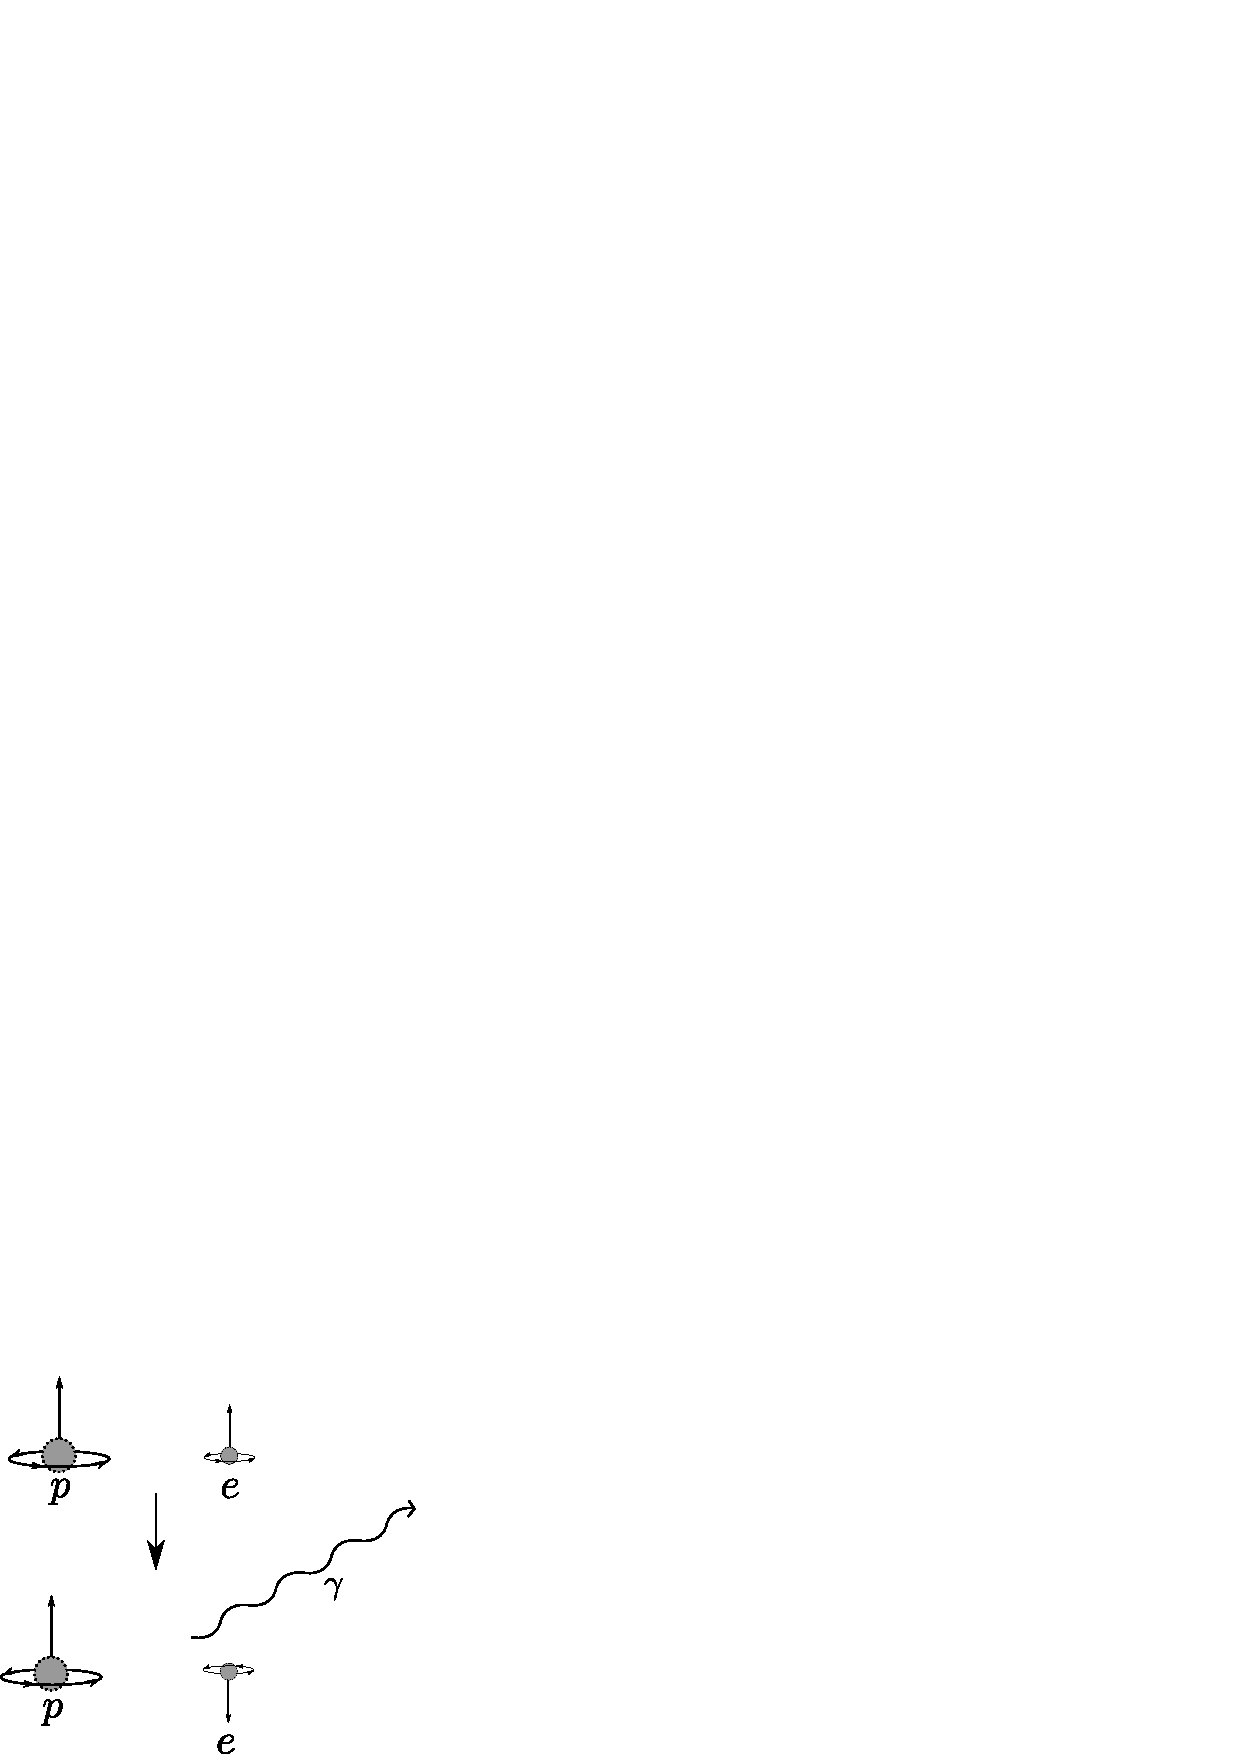
\includegraphics[width=5cm]{21cmline.pdf}
  \label{fig:21cmline}
\end{figure}
\end{columns}
\end{frame}

\begin{frame}
\frametitle{21cm Line as a Probe of Reionization}
\framesubtitle{•}
\begin{enumerate}[-]
\item Directly traces neutral hydrogen distribution
\item All-sky signal, as opposed to absorption spectra, and doesn't require a background source
\item Ability to probe higher neutral fractions than Lyman-$\alpha$ line
\item Furthermore, it could, in principle, be used to study the ``Dark Ages" prior to reionization
\end{enumerate}
\end{frame}

\begin{frame}
\frametitle{Precision Array for Probing the Epoch of Reionization}
\framesubtitle{Statistical Detection of 21cm Signal}
\begin{figure}[h]
  \centering
  \includegraphics[width=8cm]{PAPER_PS.jpg}\\
  \includegraphics[width=8cm]{PAPER_Imaging.jpg}\\
  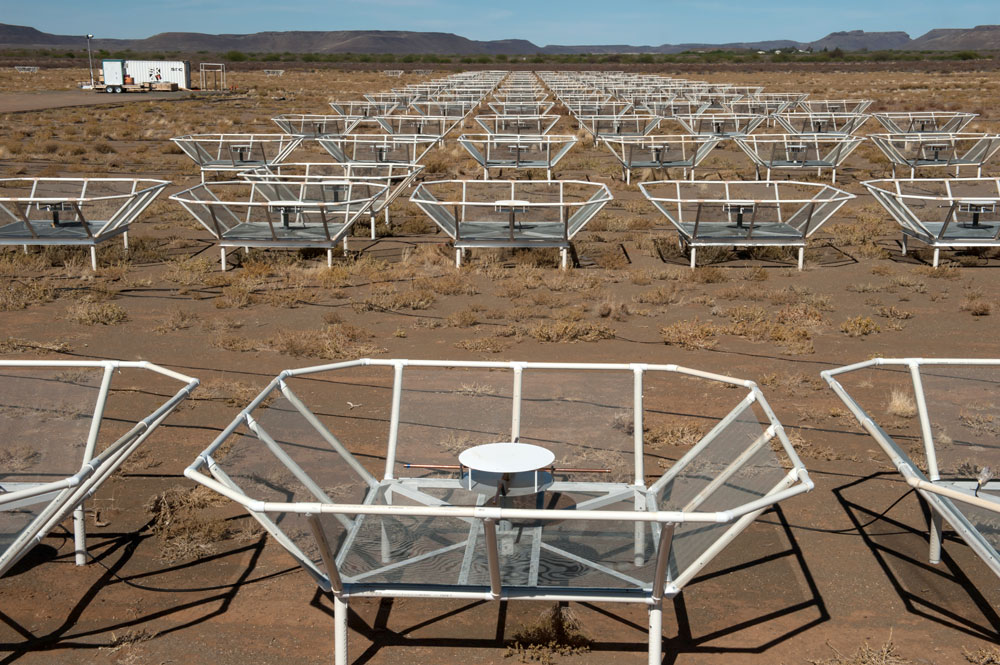
\includegraphics[width=8cm]{PAPER.jpg} 
  \caption{{\tt eor.berkeley.edu}}
  \label{fig:todo}
\end{figure}
\end{frame}

\begin{frame}
\frametitle{Giant Metrewave Radio Telescope}
\begin{figure}[h]
  \centering
  %\includegraphics[width=8cm]{GMRT_1.jpg}\\
  \includegraphics[width=8cm]{GMRT_2.jpg}
  \caption{Taken from {\tt www.mso.anu.edu.au/$\sim$plah/}, Philip Lah}
  \label{fig:todo}
\end{figure}
\end{frame}

\begin{frame}
\frametitle{Murchison Widefield Array}
\framesubtitle{•}
\begin{figure}[h]
  \centering
  \includegraphics[width=7cm]{mwanight.jpg}
  \caption{Photo found on {\tt http://www.royalsociety.org.nz}, taken by Chris Thorne.}
  \label{fig:todo}
\end{figure}
\end{frame}

\begin{frame}
\frametitle{LOw Frequency ARray}
\framesubtitle{•}
\begin{figure}[h]
  \centering
  \includegraphics[width=6cm]{LofarCore.jpg}
  \includegraphics[width=4cm]{LOFAR_Core_configuration.jpg}
  \caption{Configuration of antennae for LOFAR ({\tt www.lofar.org}).}
  \label{fig:todo}
\end{figure}
\end{frame}

%\begin{frame}
%\frametitle{21cm Line Strategies}
%\framesubtitle{Several Options}	
%\begin{enumerate}[-]
%\item 21cm Forest
%\begin{enumerate}[$\to$]
%\item Analogous to the Lyman-$\alpha$ forest. However, it is potentially more useful for studying reionization since the optical depth of the 21cm transition is much lower, allowing the line to probe deeper into the EoR without becoming saturated.
%\end{enumerate}
%\item Global 21cm Signal Measurements
%\begin{enumerate}[$\to$]
%\item Measuring the whole-sky-averaged 21cm signal as a function of frequency (redshift) can also provide information about reionization as well as formation of luminous sources prior to the EoR.
%\end{enumerate}
%\item Power spectrum of 21cm fluctuations
%\begin{enumerate}[$\to$]
%\item Shape and evolution of the 21cm power spectrum can provide much information about the progression of reionization.
%\end{enumerate}
%\end{enumerate}
%\end{frame}

\begin{frame}
\frametitle{First Generation 21cm Arrays}
\framesubtitle{Statistical Detection of 21cm Signal from EoR}
\begin{enumerate}[-]
\item First generation arrays will have low signal-to-noise per resolution element
\begin{enumerate}[$\to$]
\item As a result, the first detection of 21cm signal from EoR will likely be statistical, e.g. power spectrum measurements
\item Bin together many noise modes
\end{enumerate}
\item Power spectrum measurements can provide very useful information about the neutral fraction and bubble size distribution
\item However, the ionization field is very non-Gaussian, so the power spectrum is an incomplete description 
\end{enumerate}
\end{frame}

%
%\begin{frame}
%\frametitle{Our Focus}
%We focus on two questions. Using 2nd generation redshifted 21cm arrays, can we
%\begin{enumerate}[1.]
%\item make crude maps of the 21 cm signal?
%\begin{enumerate}[$\to$]
%\item Accurately mapping large scales can still be useful
%\end{enumerate}
%\item \textit{blindly} identify individual ionized regions?
%\begin{enumerate}[$\to$]
%\item Don't necessarily care about recovering a large fraction of underlying ionized regions 
%\item Insights can be gained from detecting a very small percentage
%\end{enumerate}
%\end{enumerate}
%\end{frame}

\begin{frame}
\frametitle{Identifying Ionized Regions}
\framesubtitle{Motivation}
\begin{enumerate}[-]
\item Identifying individual ionized regions in noisy redshifted 21cm maps can help significantly to constrain reionization.
\begin{enumerate}[$\to$]
\item Easier than making detailed maps
\end{enumerate}
\item Specifically, bubble identification can
\begin{enumerate}[$\to$]
\item provide information to remove foregrounds more accurately
\item allow targeted follow-up observations of galaxies inside/outside of ionized regions to compare/contrast their properties
%\item allow searches for a Lyman-$\alpha$ damping wing in the spectra of galaxies at the edge of bubbles in order to constrain $x_{\text{HI}}$
\item provide constraints on the neutral fraction through the average signal inside of ionized regions
\item suggest likely sources of reionization through the measured bubble size distributions.
\end{enumerate}
\end{enumerate}
\end{frame}

\begin{frame}
\frametitle{Fiducial Case}
\framesubtitle{•}
\begin{enumerate}[-]
\item Simulation
\begin{enumerate}[$\to$]
\item $L = 1\text{Gpc}/h$
\item $z_{\text{center}} = 6.9$
\item $\bar{x}_{\text{HI}} = 0.21$
\end{enumerate}
\item Noise
\begin{enumerate}[$\to$]
\item Generate mock thermal noise according to array configuration
\item Mimic the degrading effects of foreground cleaning by removing running mean along line of sight ($B = 16\text{MHz}$, $L_{\text{fg}} = 185\text{Mpc}/h$).
\end{enumerate}
\item Array configurations
\begin{enumerate}[$\to$]
\item Primarily consider scaled-up version of MWA-style instrument
\item Also consider a scaled-up version of LOFAR-style instrument
\item Representative of 2nd generation experiments
\end{enumerate}
\end{enumerate}
\end{frame}

\begin{frame}
\frametitle{Obstacles}
\framesubtitle{Life is Hard}
\begin{enumerate}[-]
\item The 21cm signal is not the only thing that contributes to measurements, there also are
\begin{enumerate}[$\to$]
\item Foregrounds
\item Thermal noise
\item Ionospheric distortions
\item Instrumental response
\end{enumerate}
\item Sources of noise can be orders of magnitude greater than the signal, for example
\begin{align*}
\delta T_{21} &\approx 28\text{mK}\ x_{\text{HI}} (1+\delta_{\rho})\left( \frac{T_{\text{S}}-T_{\text{CMB}}}{T_{\text{S}}} \right)\left( \frac{1+z}{10} \right)^{1/2} \\
T_{\text{fg}} &\sim 180\text{K} \left( \frac{\nu}{180\text{MHz}} \right)^{-2.6} \tag{Cold FOV}
\end{align*}
\end{enumerate}
\end{frame}

\begin{frame}
\frametitle{Obstacles}
\framesubtitle{Contributions to Observations}
\begin{figure}[h]
  \centering
  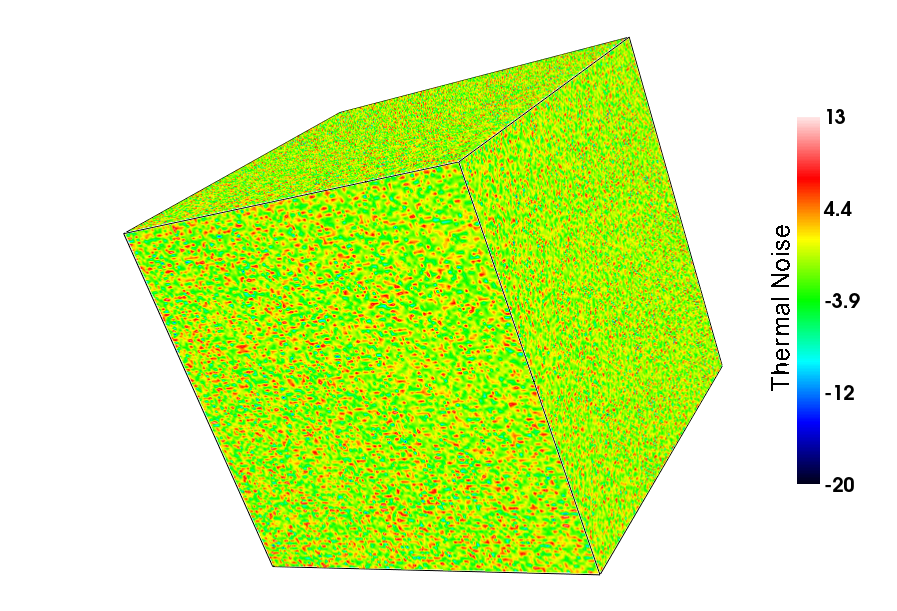
\includegraphics[width=5.3cm]{TalkNoise.png}
  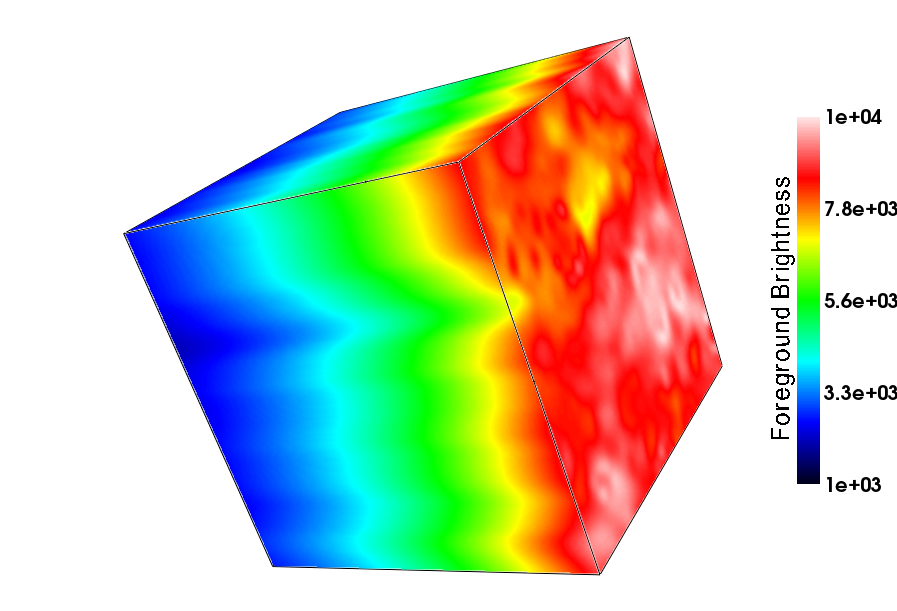
\includegraphics[width=5.3cm]{TalkFG.png}\\
  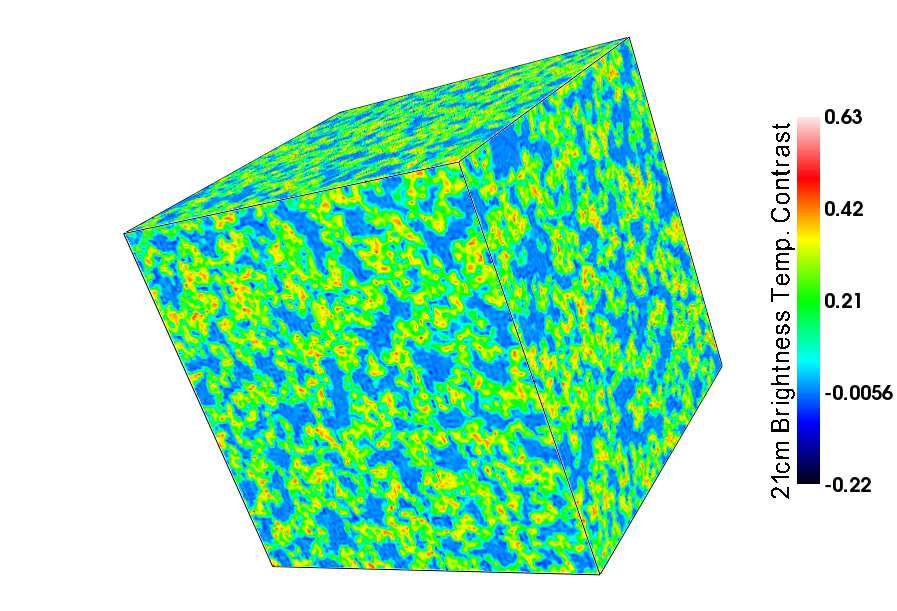
\includegraphics[width=5.3cm]{TalkSignal.png}
  \caption{todo}
  \label{fig:todo}
\end{figure}
\end{frame}


%\begin{frame}
%\frametitle{Murchison Widefield Array}
%\framesubtitle{•}
%\begin{enumerate}[-]
%\item We assume an upgraded version of the MWA experiment, consisting of 500 tiles, instead of 128.
%\end{enumerate}
%\begin{figure}[h]
%  \centering
%  \includegraphics[width=7cm]{mwanight.jpg}
%  \caption{Photo found on {\tt http://www.royalsociety.org.nz}, taken by Chris Thorne.}
%  \label{fig:todo}
%\end{figure}
%\end{frame}


%\begin{frame}
%\frametitle{LOw Frequency ARray}
%\framesubtitle{•}
%\begin{enumerate}[-]
%\item We assumed a scaled-up version of LOFAR, representative of a 2nd generation experiment with a different array configuration strategy.
%\end{enumerate}
%\begin{figure}[h]
%  \centering
%  \includegraphics[width=6cm]{LofarCore.jpg}
%  \includegraphics[width=4cm]{LOFAR_Core_configuration.jpg}
%  \caption{Configuration of antennae for LOFAR ({\tt www.lofar.org}).}
%  \label{fig:todo}
%\end{figure}
%\end{frame}

%\begin{frame}
%\frametitle{Recovering 21cm Maps}
%\framesubtitle{Wiener Filter}
%\begin{enumerate}[-]
%\item First, we utilized a Wiener filter to assess the ability of an upgraded MWA to make maps of the 21 cm signal.
%\item Wiener filter is optimal for recovering a signal corrupted by additive noise.
%\begin{enumerate}[$\to$]
%\item Minimizes the expected squared error between the original signal and recovered signal.
%\item Allows at least partial recovery of underlying signal as long as the signal dominates the noise for some (Fourier) $k$-modes.
%\item In our case, the filter takes the form (in Fourier space):
%\begin{equation}
%W(k,\mu) = \frac{P_{\text{S}}(k)}{P_{\text{S}}(k) + P_{\text{N}}(k,\mu)}.
%\end{equation}
%\end{enumerate}
%\end{enumerate}
%\end{frame}
%
%\begin{frame}
%\frametitle{Recovering 21cm Maps: Results}
%\begin{figure}[h]
%  \centering
%  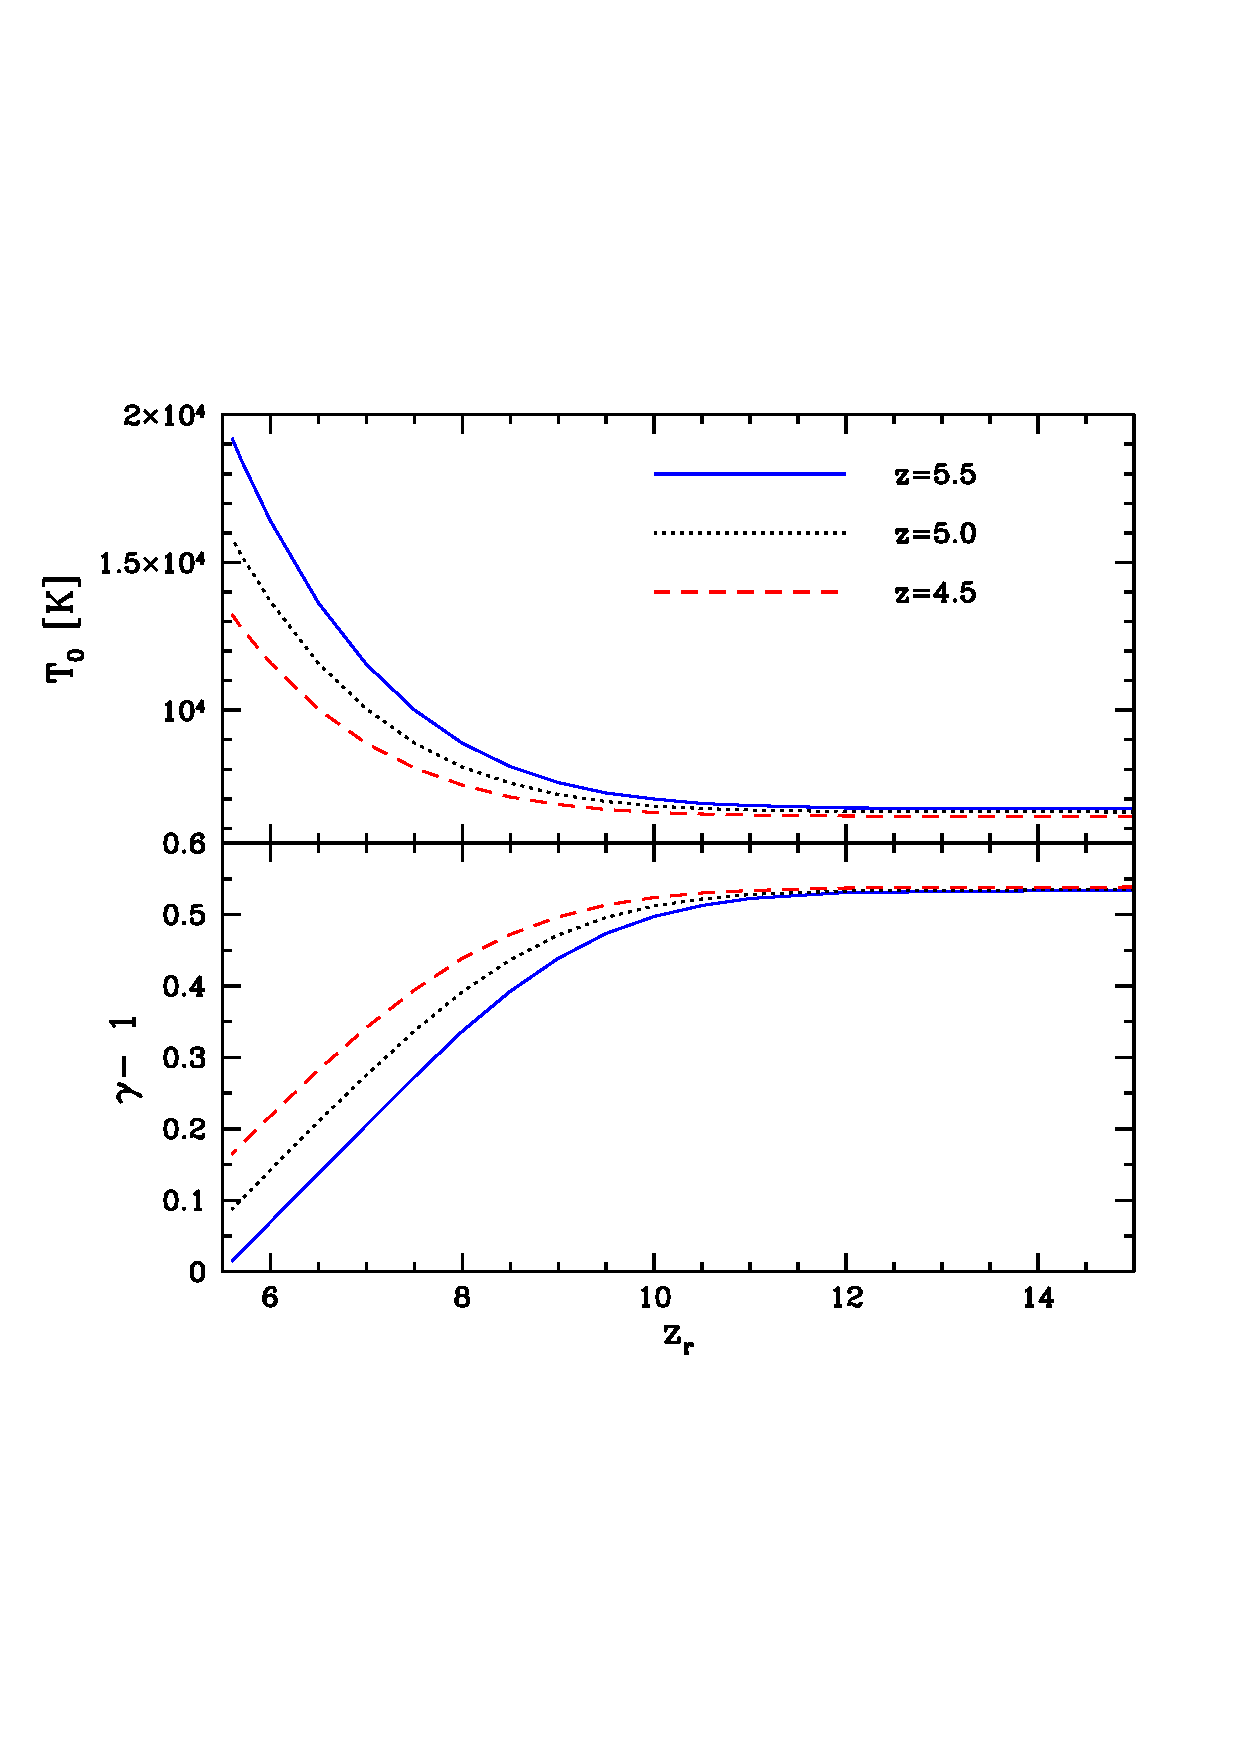
\includegraphics[width=9cm]{f2.png}
%  %\caption{Results of applying the Wiener filter to noisy 21cm data (MWA-500)}
%  \label{fig:todo}
%\end{figure}
%\end{frame}

%\begin{frame}
%\frametitle{Identifying Ionized Regions}
%\framesubtitle{Motivation}
%\begin{enumerate}[-]
%\item Identifying individual ionized regions in noisy redshifted 21cm maps can help significantly to constrain reionization.
%\begin{enumerate}[$\to$]
%\item Easier than making detailed maps
%\end{enumerate}
%\item Specifically, bubble identification can
%\begin{enumerate}[$\to$]
%\item provide information to remove foregrounds more accurately
%\item allow targeted follow-up observations of galaxies inside/outside of ionized regions to compare/contrast their properties
%%\item allow searches for a Lyman-$\alpha$ damping wing in the spectra of galaxies at the edge of bubbles in order to constrain $x_{\text{HI}}$
%\item provide constraints on the neutral fraction through the average signal inside of ionized regions
%\item suggest likely sources of reionization through the measured bubble size distributions.
%\end{enumerate}
%\end{enumerate}
%\end{frame}

\begin{frame}
\frametitle{Identifying Ionized Regions}
\framesubtitle{Optimal Matched Filter}
\begin{enumerate}[-]
\item In the case where you have a known feature embedded in noise, the filter that maximizes your signal-to-noise (SNR) when detecting the feature is the \textit{optimal matched filter}.
\item The filters acts by convolving the noisy signal with a template of the known feature and by downweighting noisy modes. 
\begin{equation}
M(k,\mu) = \frac{T(k)}{P_{\text{N}}(k,\mu)} \to \frac{T(k;R)}{P_{\text{N}}(k,\mu)}
\end{equation}
\begin{enumerate}[$\implies$]
\item This implies constructing the filter involves specifying a template, $T(k)$, and approximately knowing the noise power, $P_{\text{N}}(k,\mu)$.
\end{enumerate}
\item Although ionized regions are manifestly not spherical, we find a spherical top-hat with a variable radius ($T(k;R)$) is an effective choice. 
\end{enumerate}
\end{frame}

\begin{frame}
\frametitle{Optimal Matched Filter}
\begin{figure}[h]
  \centering
  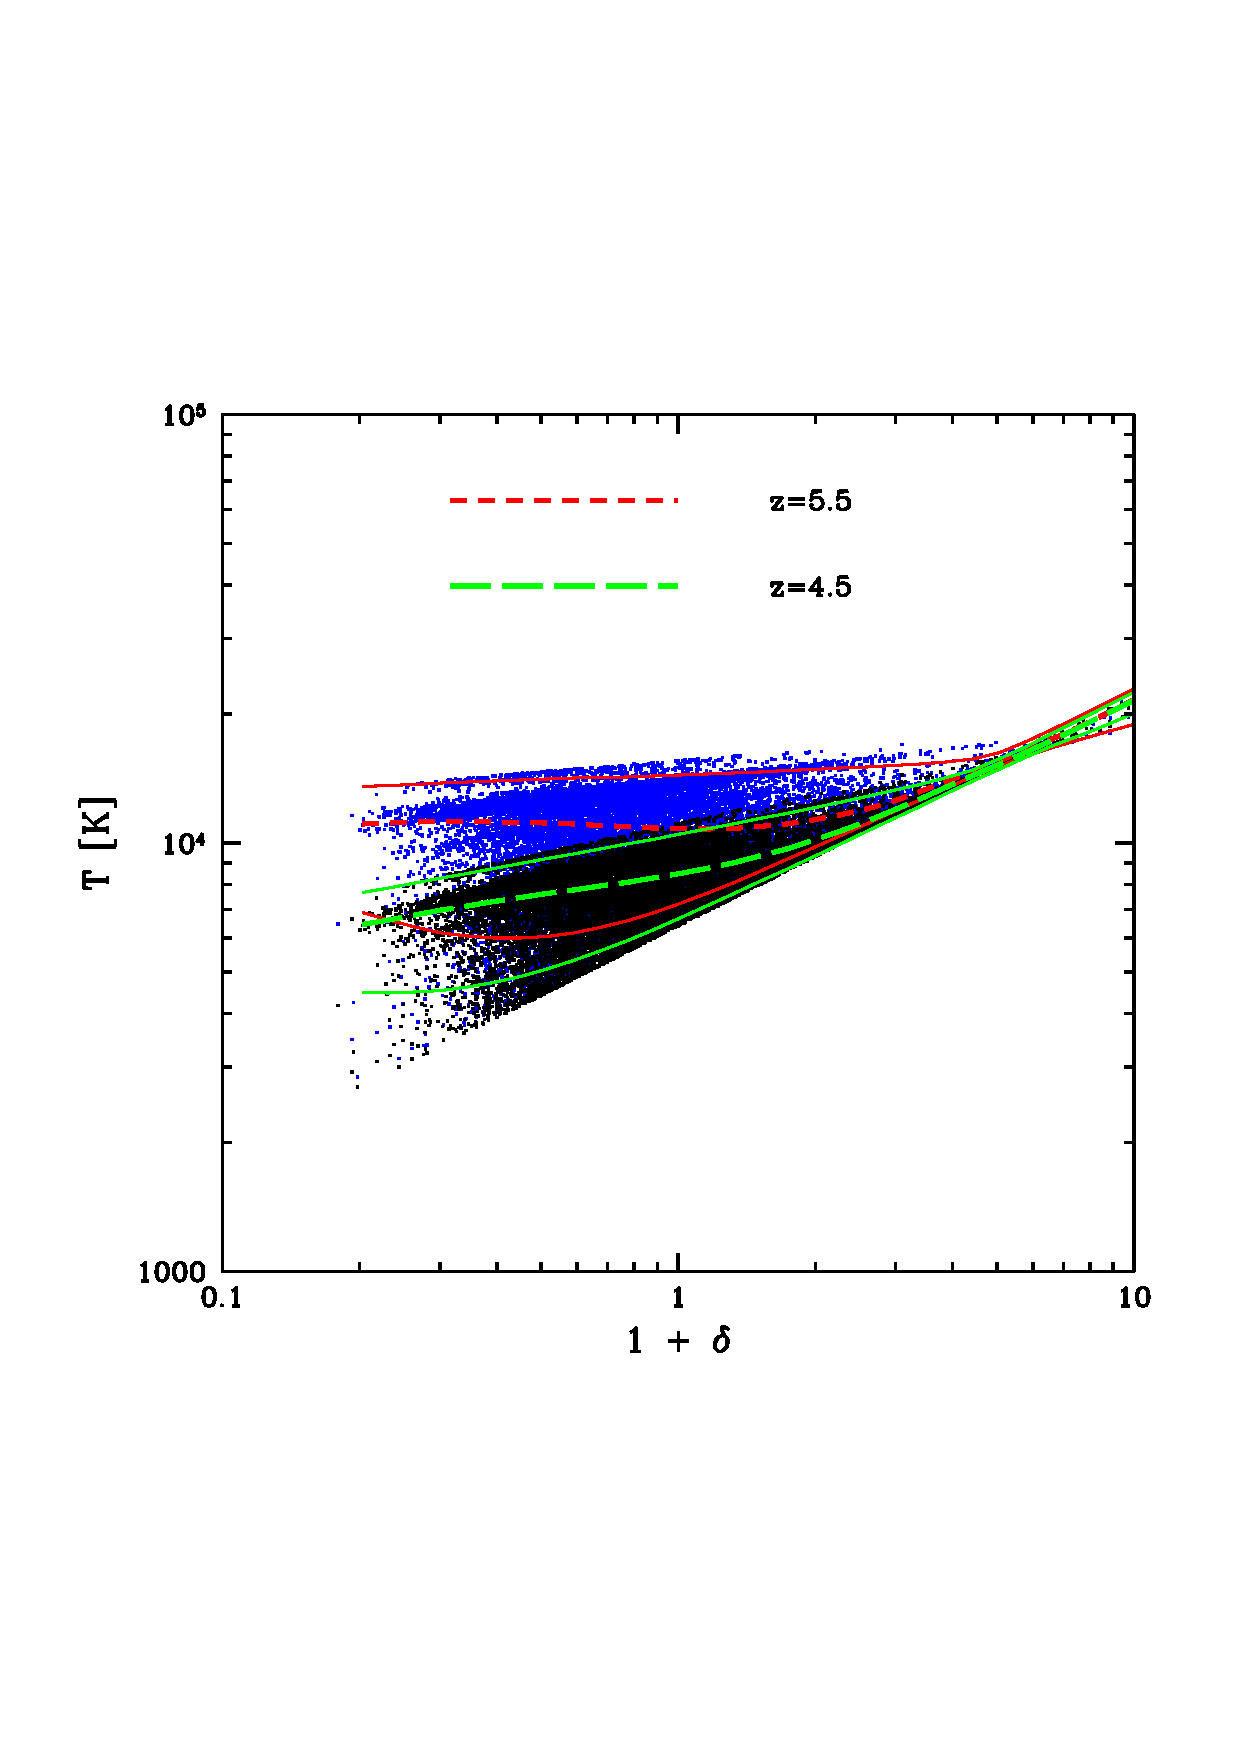
\includegraphics[width=9cm]{f5.png}
  %\caption{todo}
\end{figure}
\end{frame}

\begin{frame}
\frametitle{Identifying Ionized Regions}
\framesubtitle{Algorithm}
\begin{enumerate}[1.]
\item[] When $R_{\text{template}} = R_{\text{Bubble}}$, then SNR is maximized for isolated spherical bubbles. Using this, we:
%\item[] For an isolated, spherical ionized region, the SNR value will be maximized when the template radius of the matched filter matches the radius of the ionized region. 
\item Vary template radius over physically-relevant interval $R_{\min} \leq R_{\text{template}} \leq R_{\max}$.
%\item We apply the matched filter to the data repeatedly while varying the radius of the template over a physically-relevant interval.
\item Track maximum SNR value at \textit{each} pixel.
%\item We keep track of the maximum SNR value attained by \textit{each} pixel in the data cube over the entire range of template radii.
\item Construct a new field where each pixel is given its corresponding maximum SNR value.
\item Local maxima in this field are the centers of candidate bubbles.
\item Candidate bubble's radius is the template radius that maximized the pixel's SNR.
\item Throw out all bubbles with $\text{SNR} < \text{SNR}_{\min}$.
\end{enumerate}
\end{frame}


\begin{frame}
\frametitle{Identified Bubble Example}
\framesubtitle{}
\begin{figure}[h]
  \centering
  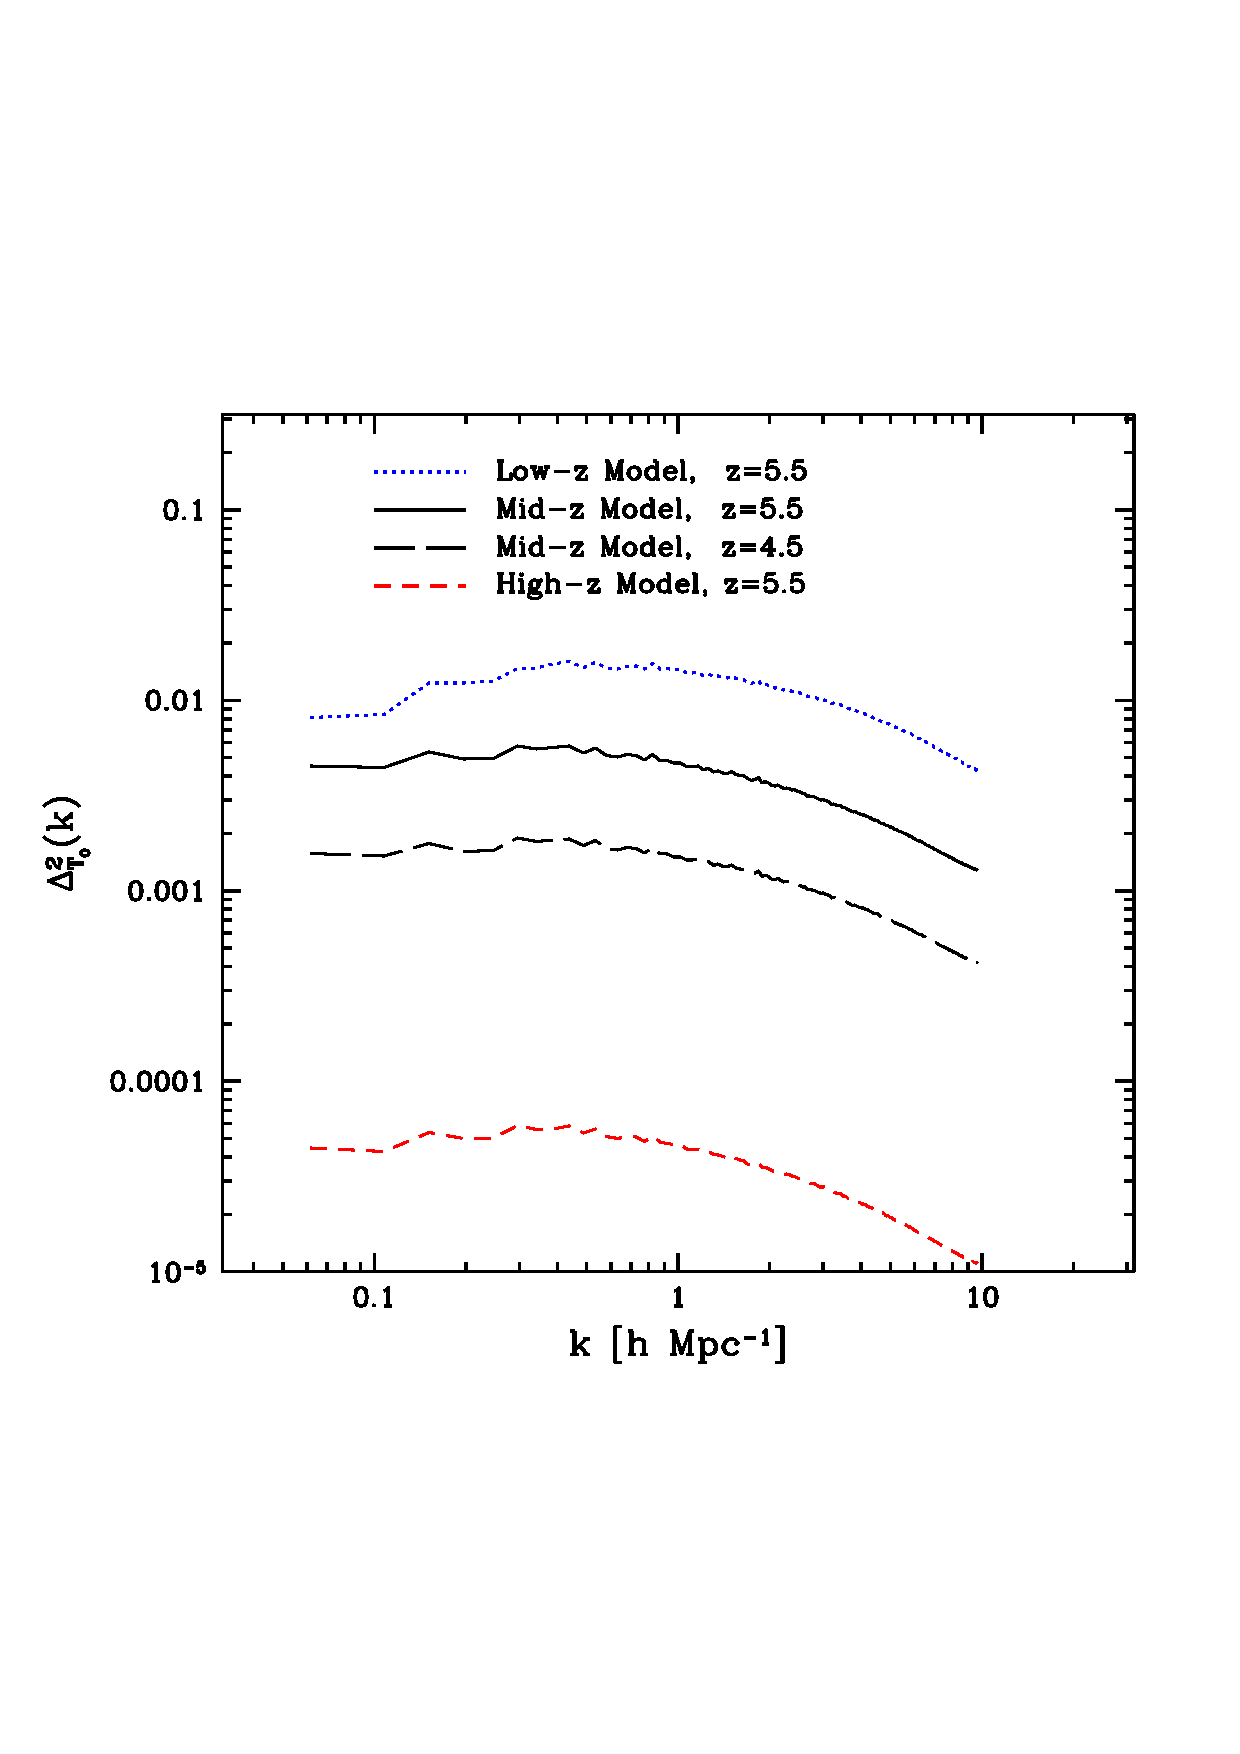
\includegraphics[width=9cm]{f7.png}
\end{figure}
\end{frame}

\begin{frame}
\frametitle{Detecting a Single Bubble as Multiple}
\begin{figure}[h]
  \centering
  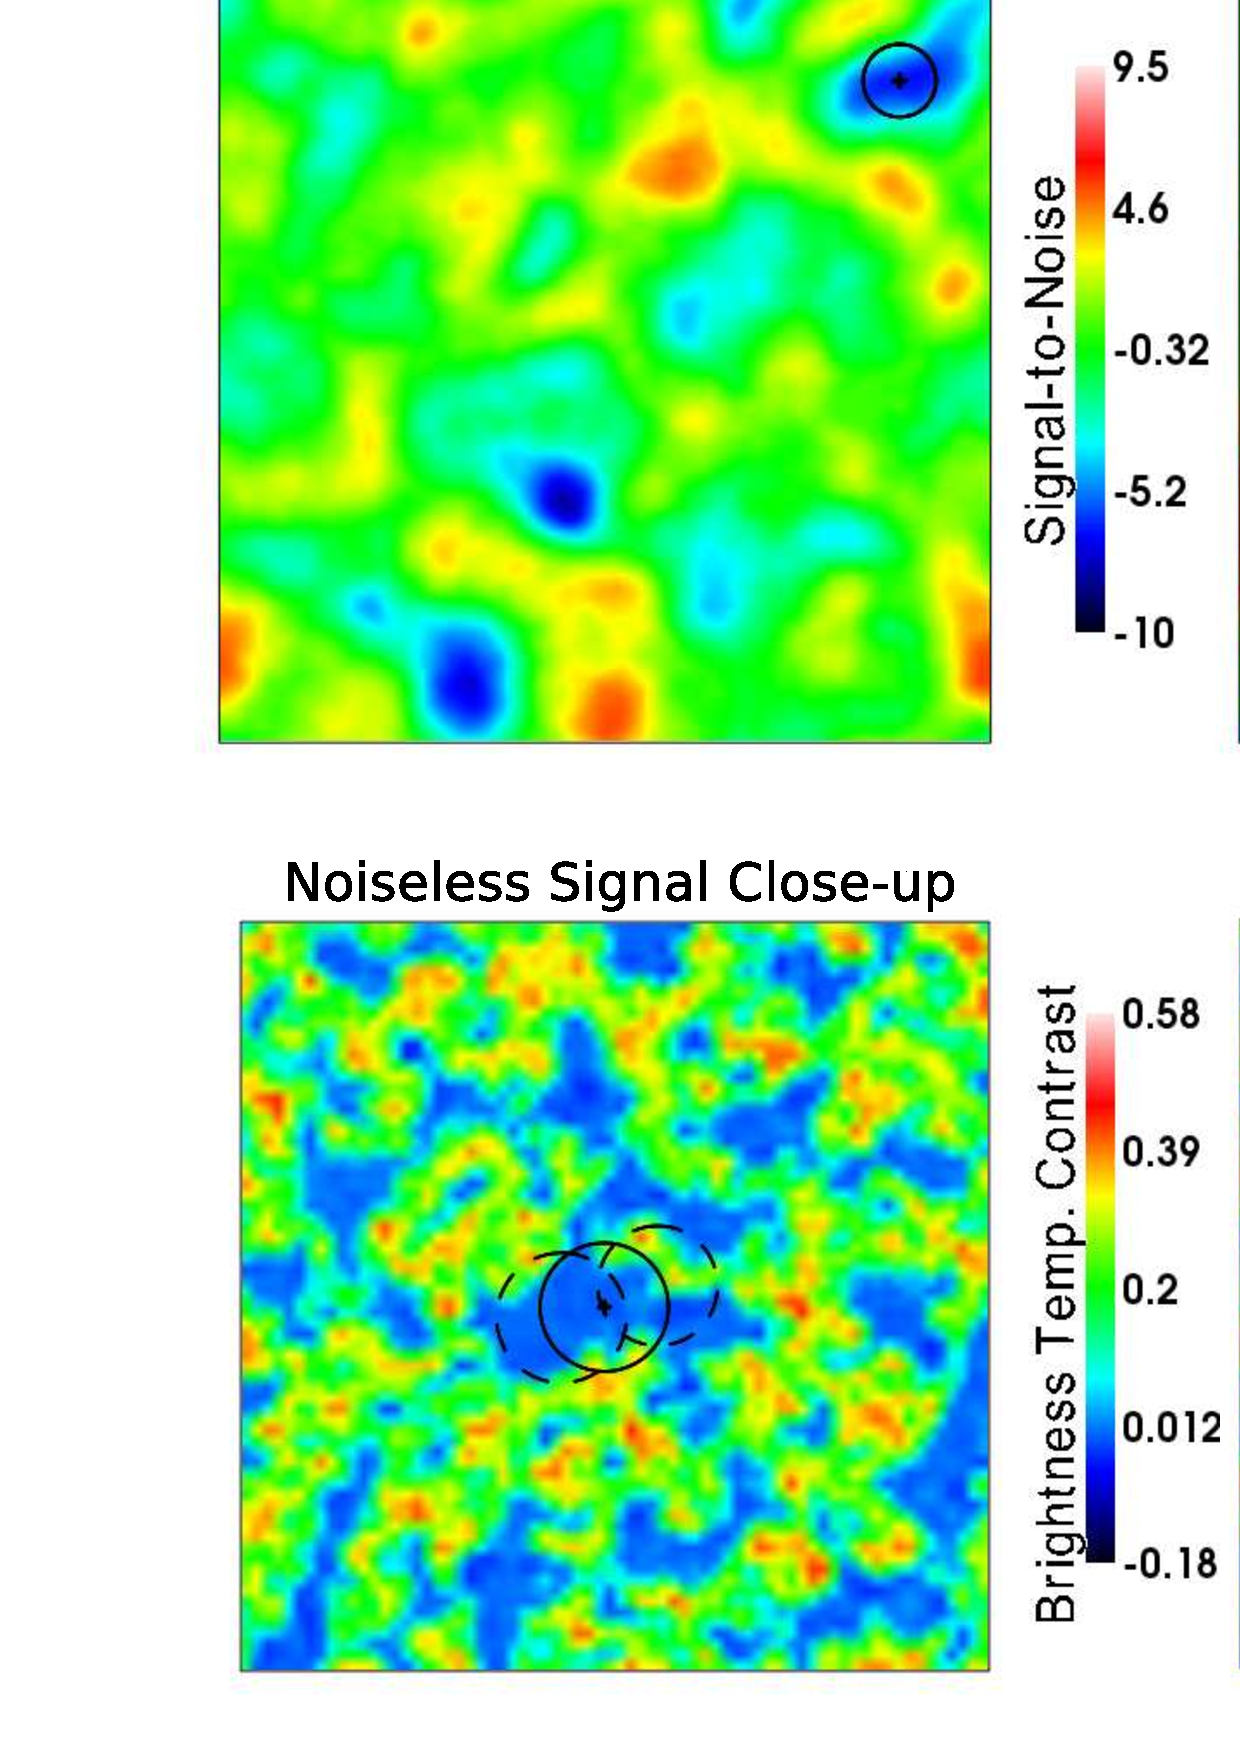
\includegraphics[width=9cm]{f8.png}
\end{figure}
\end{frame}

\begin{frame}
\frametitle{Success of Detected Bubbles}
\framesubtitle{•}
\begin{enumerate}[-]
\item For our fiducial reionization simulation ($L = 1\gpch$, $x_{\text{HI}} = 0.21$, $z = 6.90$) we detect $\sim$220 bubbles ($\sim140$ when rescaled to MWA survey volume).
\item $\sim$96\% of bubbles are more ionized than the simulation box on average.
\item $\sim$43\% of bubbles are more than 90\% ionized.
\end{enumerate}
\begin{figure}[h]
  \centering
  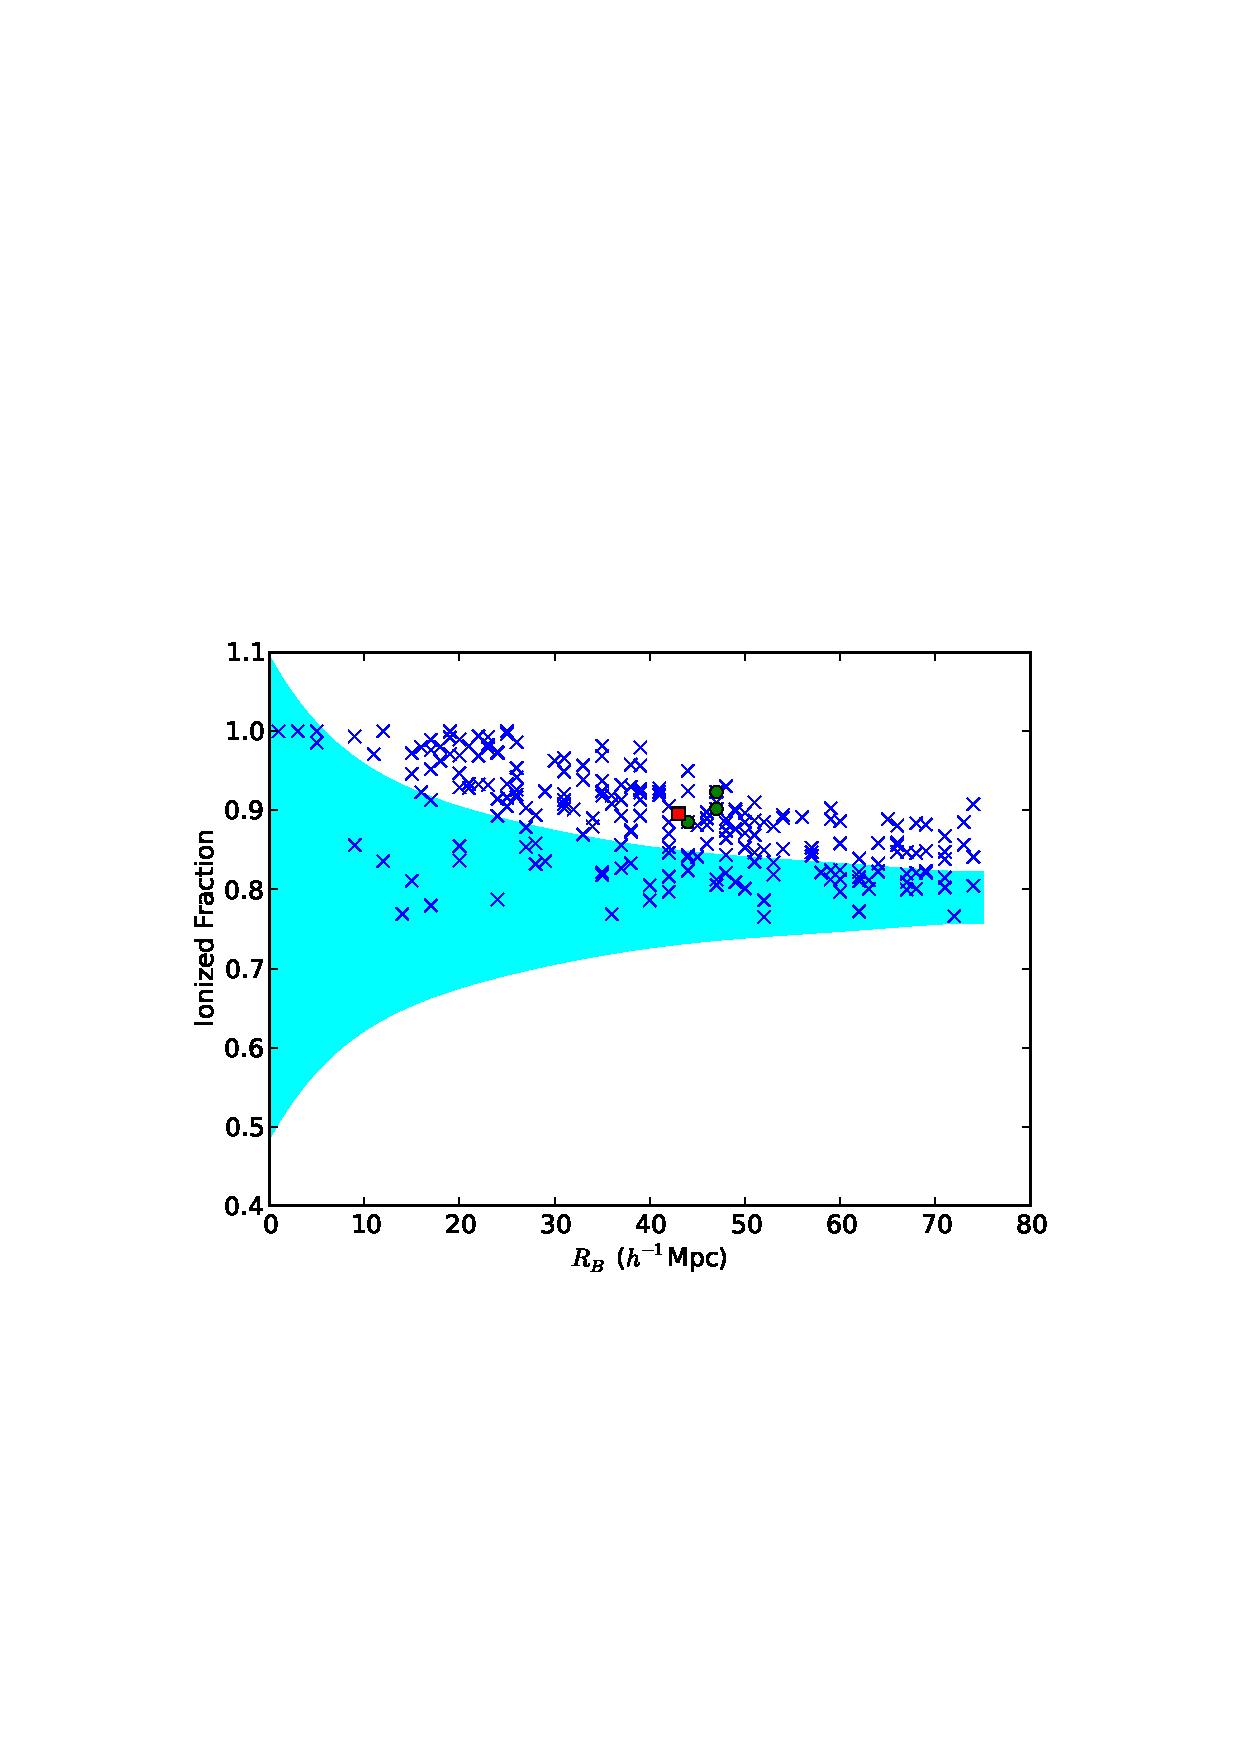
\includegraphics[width=7cm]{f9.png}
\end{figure}
\end{frame}

\begin{frame}
\frametitle{Summary}
\framesubtitle{}
\begin{enumerate}[-]
\item Bubble detection should be successful with second generation arrays, provided systematic effects can be mitigated
\item This would open up several interesting avenues for constraining neutral fraction
\item ({\tt arXiv:1212.2656})
\end{enumerate}
\end{frame}

\begin{frame}
\frametitle{Future Work}
\framesubtitle{More Realistic Bubble Detection}
\begin{figure}[h]
  \centering
  \includegraphics[width=6cm]{ASU.png}
\end{figure}
\begin{enumerate}[-]
\item Currently teaming up with Judd Bowman, Piyanat Kittiwisit, and Daniel Jacobs
\item Working on applying bubble detection algorithm to 21cm signals corrupted by more realistic foregrounds and noise
\begin{enumerate}[$\to$]
\item Are we still able to detect bubbles?
\item Can we use the average signal in bubbles to accurately constrain $x_{\text{HI}}$?
\end{enumerate}
\end{enumerate}
\end{frame}

\begin{frame}
\frametitle{Future Work}
\framesubtitle{Global 21cm Signal and Matched Filtering}
Global 21cm signal also contains much information about structure formation and reionization.\\
%\item Points $A$, $B$, $C$, $D$, and $E$ generic predictions of structure formation models.
$\delta T_{21} = 28 x_{\text{HI}}(1+\delta) \left( \frac{T_{\text{S}} - T_{\text{CMB}}}{T_{\text{S}}} \right)\left( \frac{1+z}{10} \right)^{1/2}\text{mK}$
\begin{columns}[l]
\column{2.3in}
$A$: Collisions become inefficient at coupling $T_{\text{S}} \to T_{K}$.\\
$B$: First stars turn on\\
$C$: First X-ray sources turn on\\
$D$: 21cm signal saturates, reionization begins\\
$E$: EoR completes, $\delta T_{21}\to 0$\\
\column{1.8in}
\begin{figure}[h]
  \centering
  \includegraphics[width=4cm]{harker.png}
  \caption{{\tiny \cite{Harker:2011et}}}
\end{figure}
\end{columns}
\end{frame}

\begin{frame}
\frametitle{Future Work}
\framesubtitle{Global 21cm Signal and Matched Filtering}
Global 21cm signal also contains much information about structure formation and reionization.\\
%\item Points $A$, $B$, $C$, $D$, and $E$ generic predictions of structure formation models.
$\delta T_{21} = 28 x_{\text{HI}}(1+\delta) \left( \frac{T_{\text{S}} - T_{\text{CMB}}}{T_{\text{S}}} \right)\left( \frac{1+z}{10} \right)^{1/2}\text{mK}$
\begin{columns}[l]
\column{2.3in}
\begin{enumerate}[-]
\item Seems easier since you only need the \textit{sky-averaged} signal
\item However, this signal will be buried in foregrounds
\item Global signal evolves much more smoothly along line of sight than fluctuation signal
\begin{enumerate}[$\to$]
\item Foreground subtraction becomes a bigger problem
\end{enumerate}
\end{enumerate} 
%$A$: Collisions become inefficient at coupling $T_{\text{S}} \to T_{K}$.\\
%$B$: First stars turn on\\
%$C$: First X-ray sources turn on\\
%$D$: 21cm signal saturates, reionization begins\\
%$E$: EoR completes, $\delta T_{21}\to 0$\\
\column{1.8in}
\begin{figure}[h]
  \centering
  \includegraphics[width=4cm]{harker.png}
  \caption{{\tiny \cite{Harker:2011et}}}
\end{figure}
\end{columns}
\end{frame}

\begin{frame}
\frametitle{Future Work}
\framesubtitle{Global 21cm Signal and Matched Filtering}
\begin{enumerate}[-]
\item Model of structure formation predicts a certain $\delta T_{21}(z)$ curve.
\begin{enumerate}[$\to$]
\item Ideal application for a matched filter.
\item Can using an array of template functions allow us to estimate the most likely $\delta T_{21}(z)$ curve? Constrain timing of turning points $A-E$?
\end{enumerate}
\item One experiment being proposed is Dark Ages Radio Explorer (DARE).
\end{enumerate}
\begin{figure}[h]
  \centering
  \includegraphics[width=5cm]{DareWindow.jpg}
  \includegraphics[width=4cm]{WaitWhatTheMoon.png}
  \caption{{\tt lunar.colorado.edu}}
  \label{fig:todo}
\end{figure}
\end{frame}

\begin{frame}
\frametitle{Future Work}
\framesubtitle{High-$z$ Quasar Spectra and Matched Filtering}
%\animategraphics[autoplay,loop,height=5cm]{5}{0polar}{0}{24}
%\animategraphics[autoplay,loop,height=5cm]{5}{ETauVsZ_LOS1_}{1}{20}
\ \ \ \ \ \animategraphics[autoplay,loop,height=3cm]{5}{Talk_}{1}{20}
\begin{flushleft}
\begin{figure}
  \includegraphics[width=10.7cm]{Ion.png}
\end{figure}
\end{flushleft}
%\column{1.8in}
%\animategraphics[autoplay,loop,height=5cm]{5}{polar}{0}{17}
%\indent {\tiny Look at me, made an animation all on my own.}
\end{frame}

\begin{frame}
\frametitle{Conclusions}
\framesubtitle{•}
\begin{enumerate}[-]
\item Reionization is an important, yet only loosely-constrained, process in Universe's history
\item A wide variety of strategies exist for putting constraints on the process, yet many await future data
\item While some data and constraints already exist, several hotly-anticipated reionization experiments are gearing up to collect data over the next decade
\end{enumerate}
\end{frame}

\begin{frame}
\frametitle{Conclusions}
\framesubtitle{•}
\begin{enumerate}[-]
\item Reionization is an important, yet only loosely-constrained, process in Universe's history
\item A wide variety of strategies exist for putting constraints on the process, yet many await future data
\item While some data and constraints already exist, several hotly-anticipated reionization experiments are gearing up to collect data over the next decade
\end{enumerate}
\begin{center}
{\LARGE Thank you!}
\end{center}
\end{frame}

%%%%%%%%% BACKUP SLIDES %%%%%%%%%%%%%

\begin{frame}
\frametitle{Comparing Arrays}
\begin{figure}[h]
  \centering
  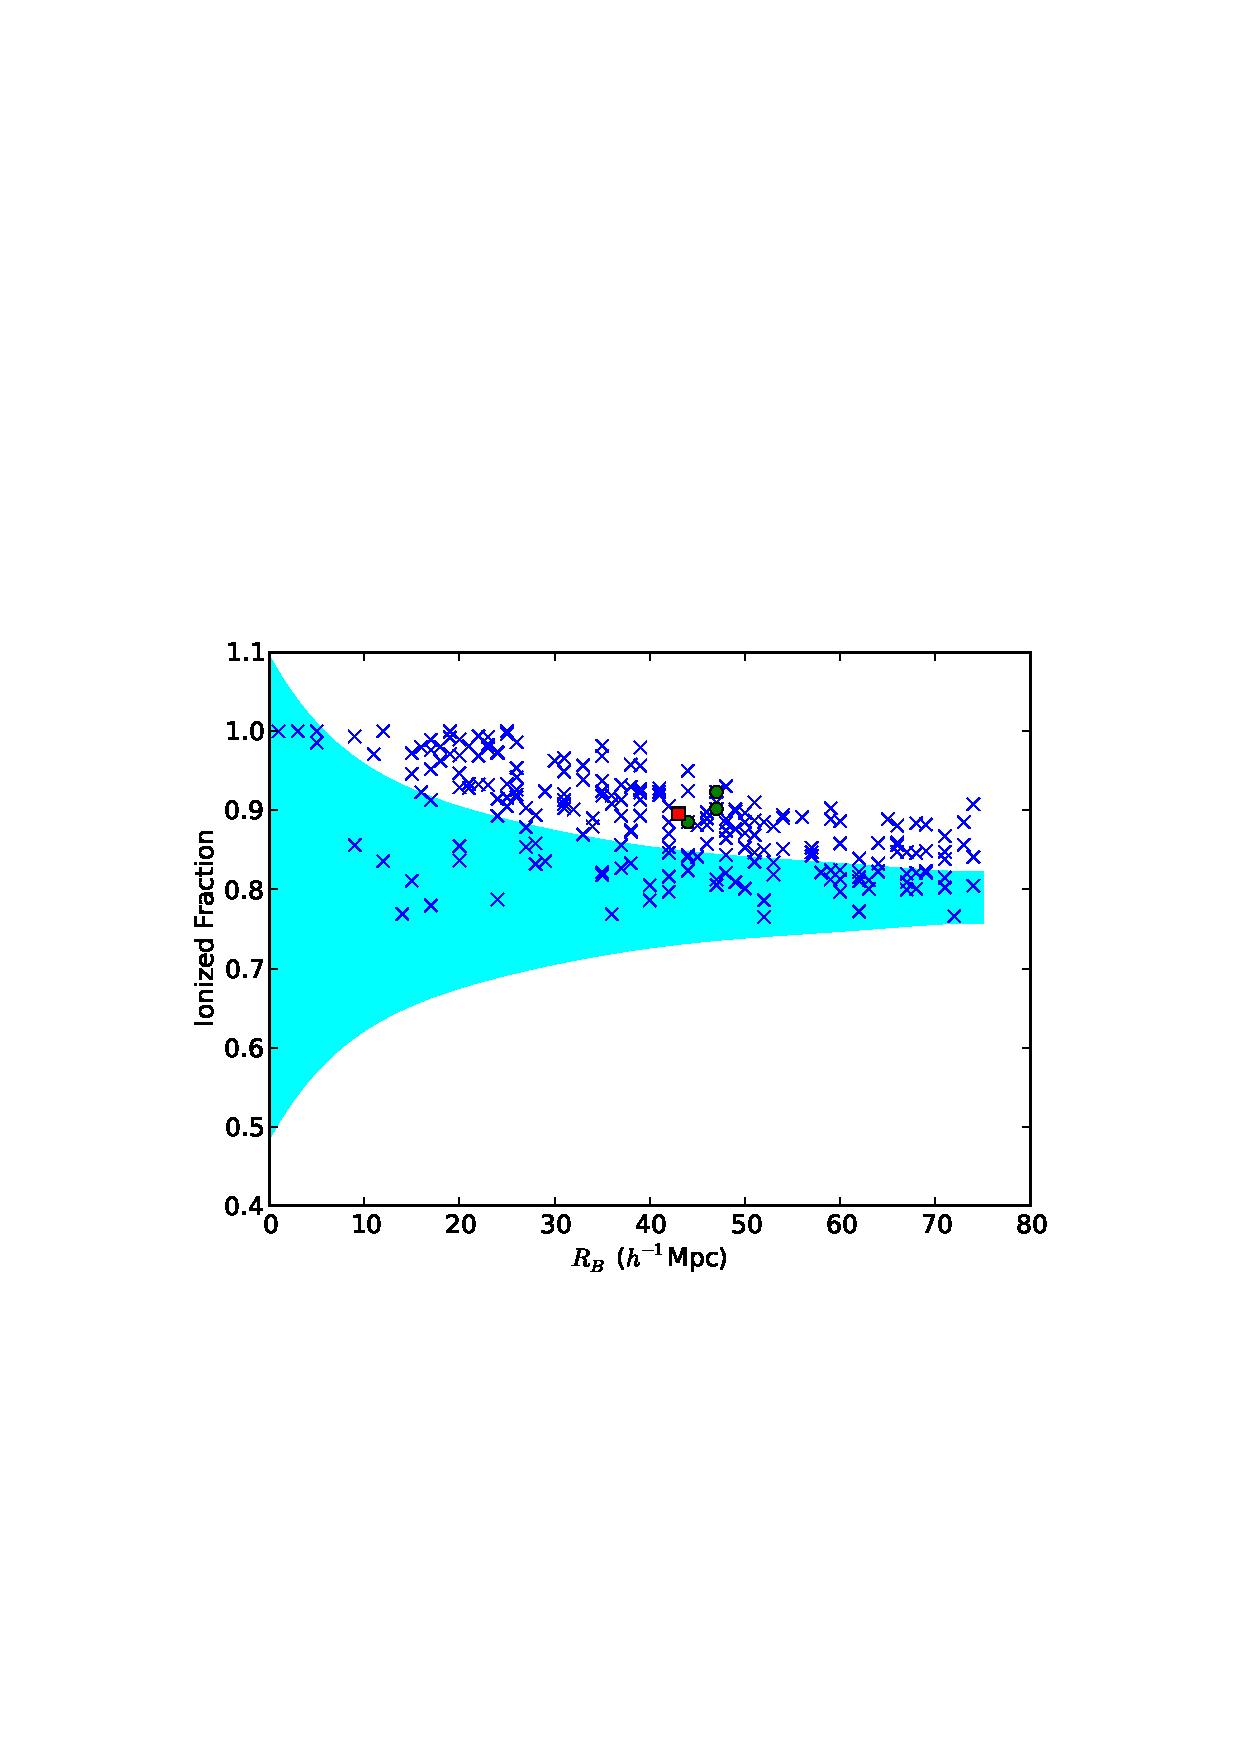
\includegraphics[width=5cm]{f9.png}
  \includegraphics[width=5cm]{successMWA128.png}\\
  \includegraphics[width=5cm]{successLOFAR.png}
\end{figure}
\end{frame}

\begin{frame}
\frametitle{Wiener Filter Fourier Profile (Back-up Slides Begin Here)}
\framesubtitle{•}
\begin{figure}[h]
  \centering
  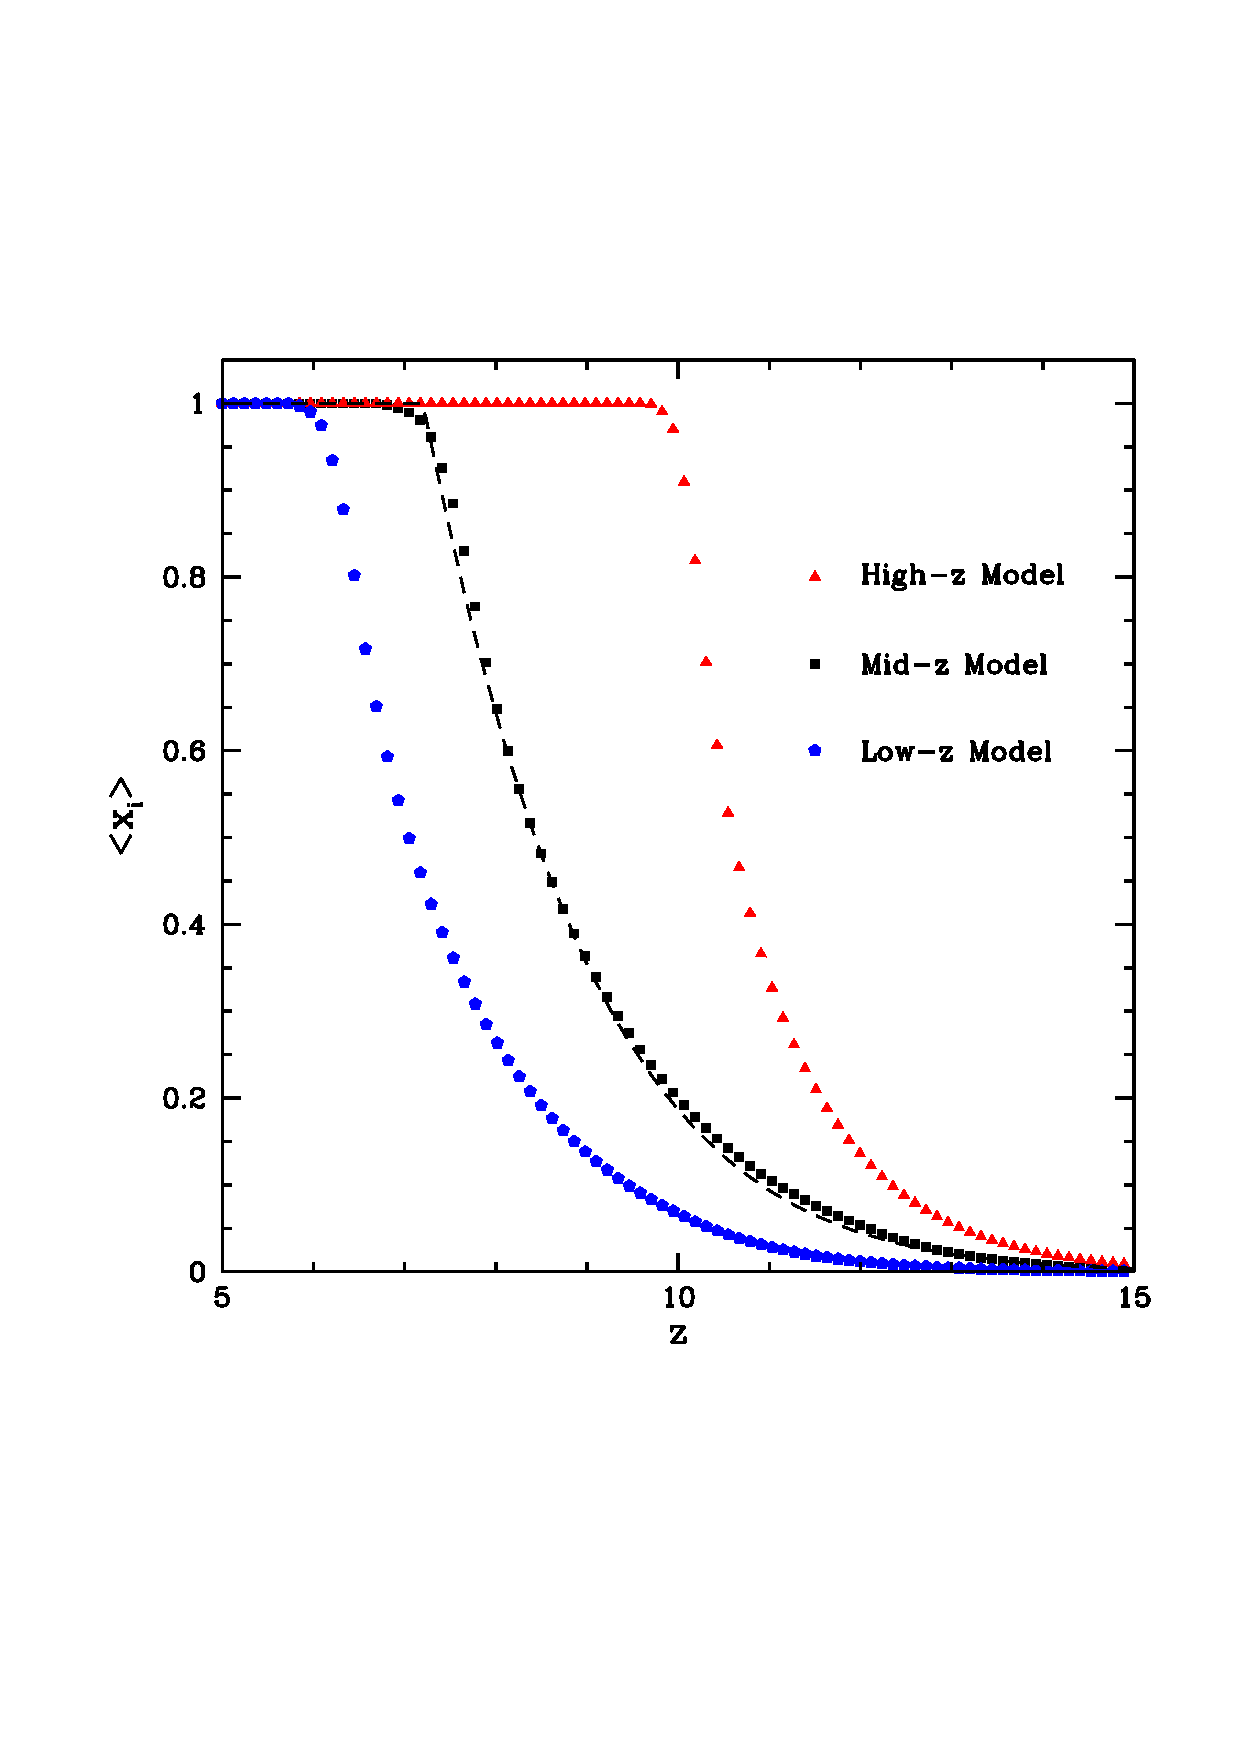
\includegraphics[width=8cm]{f1.png}
\end{figure}
\end{frame}

\begin{frame}
\frametitle{Effects of Foreground Cleaning on Imaging}
\framesubtitle{•}
\begin{figure}[h]
  \centering
  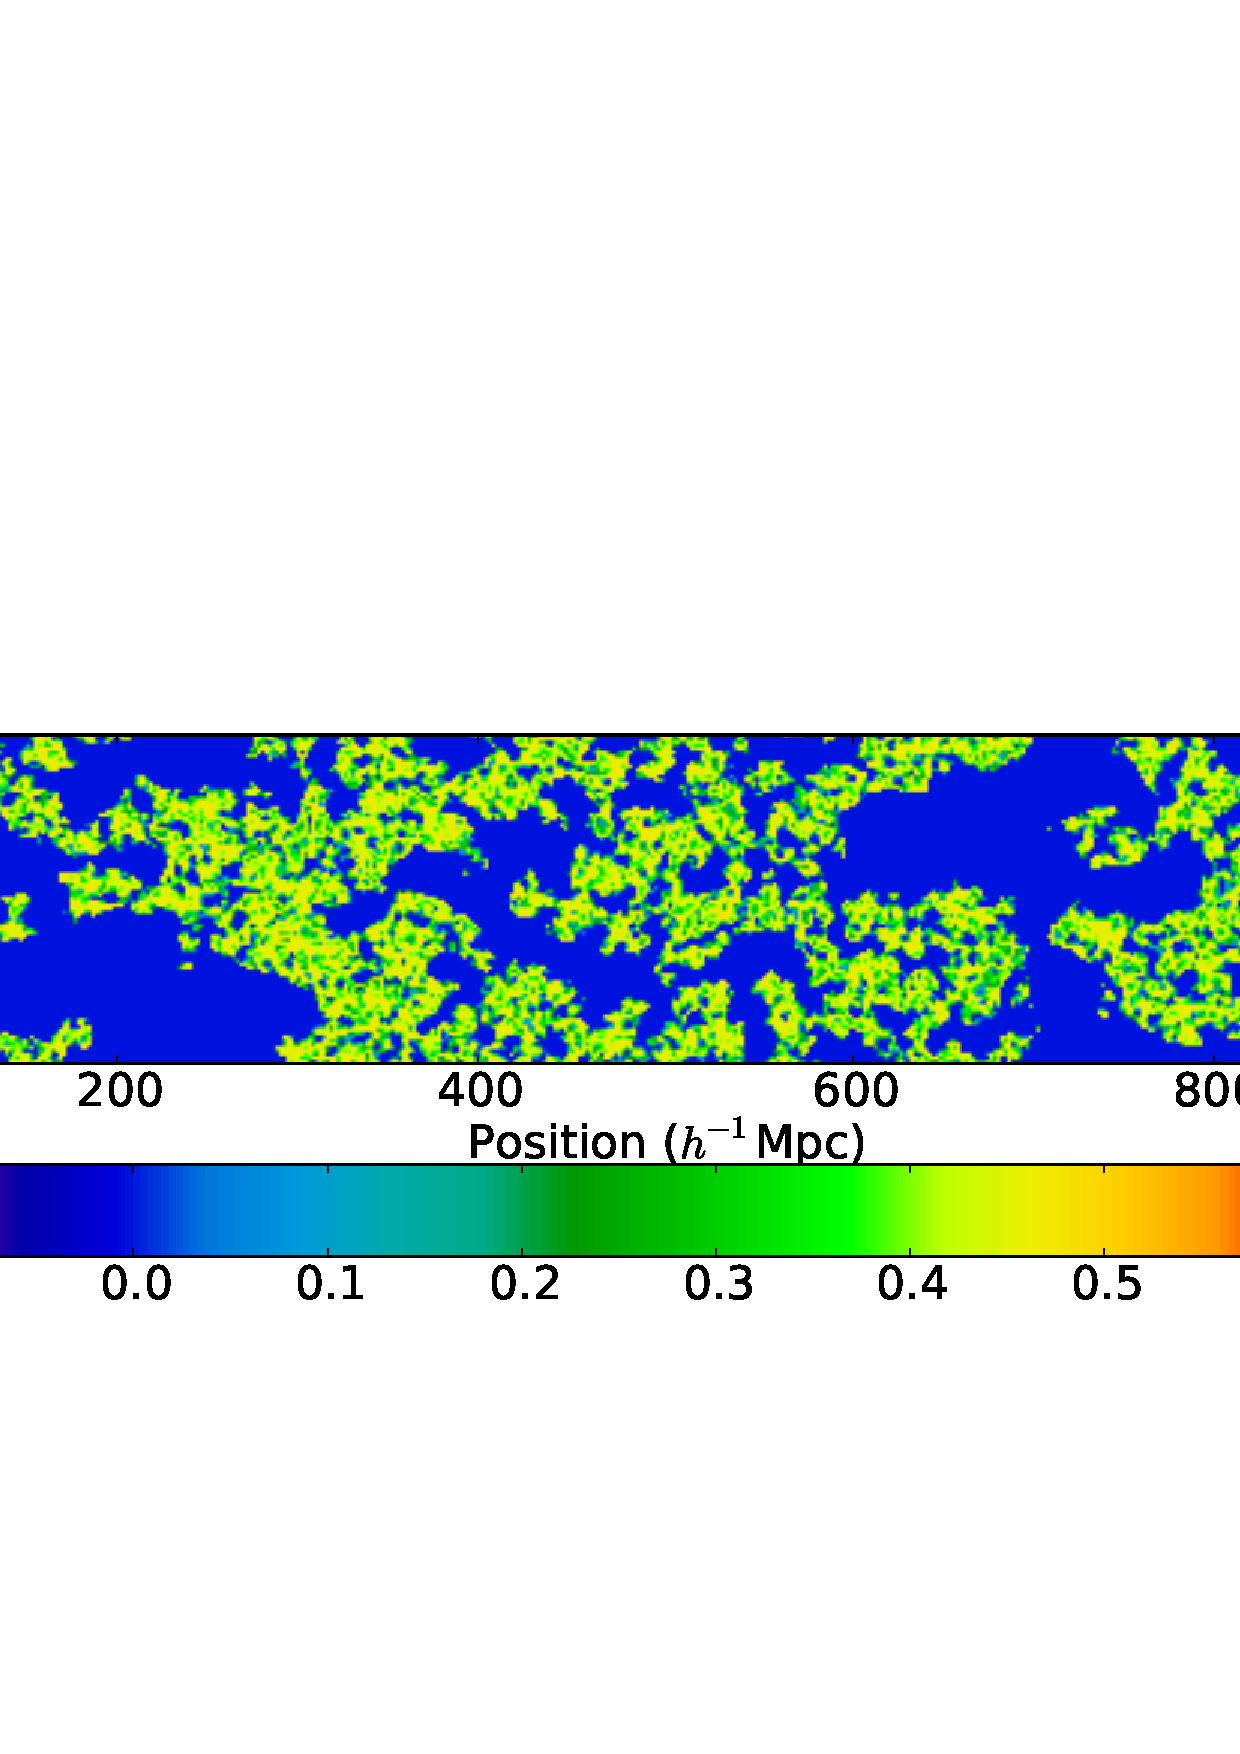
\includegraphics[width=8cm]{f3a.png}\\
  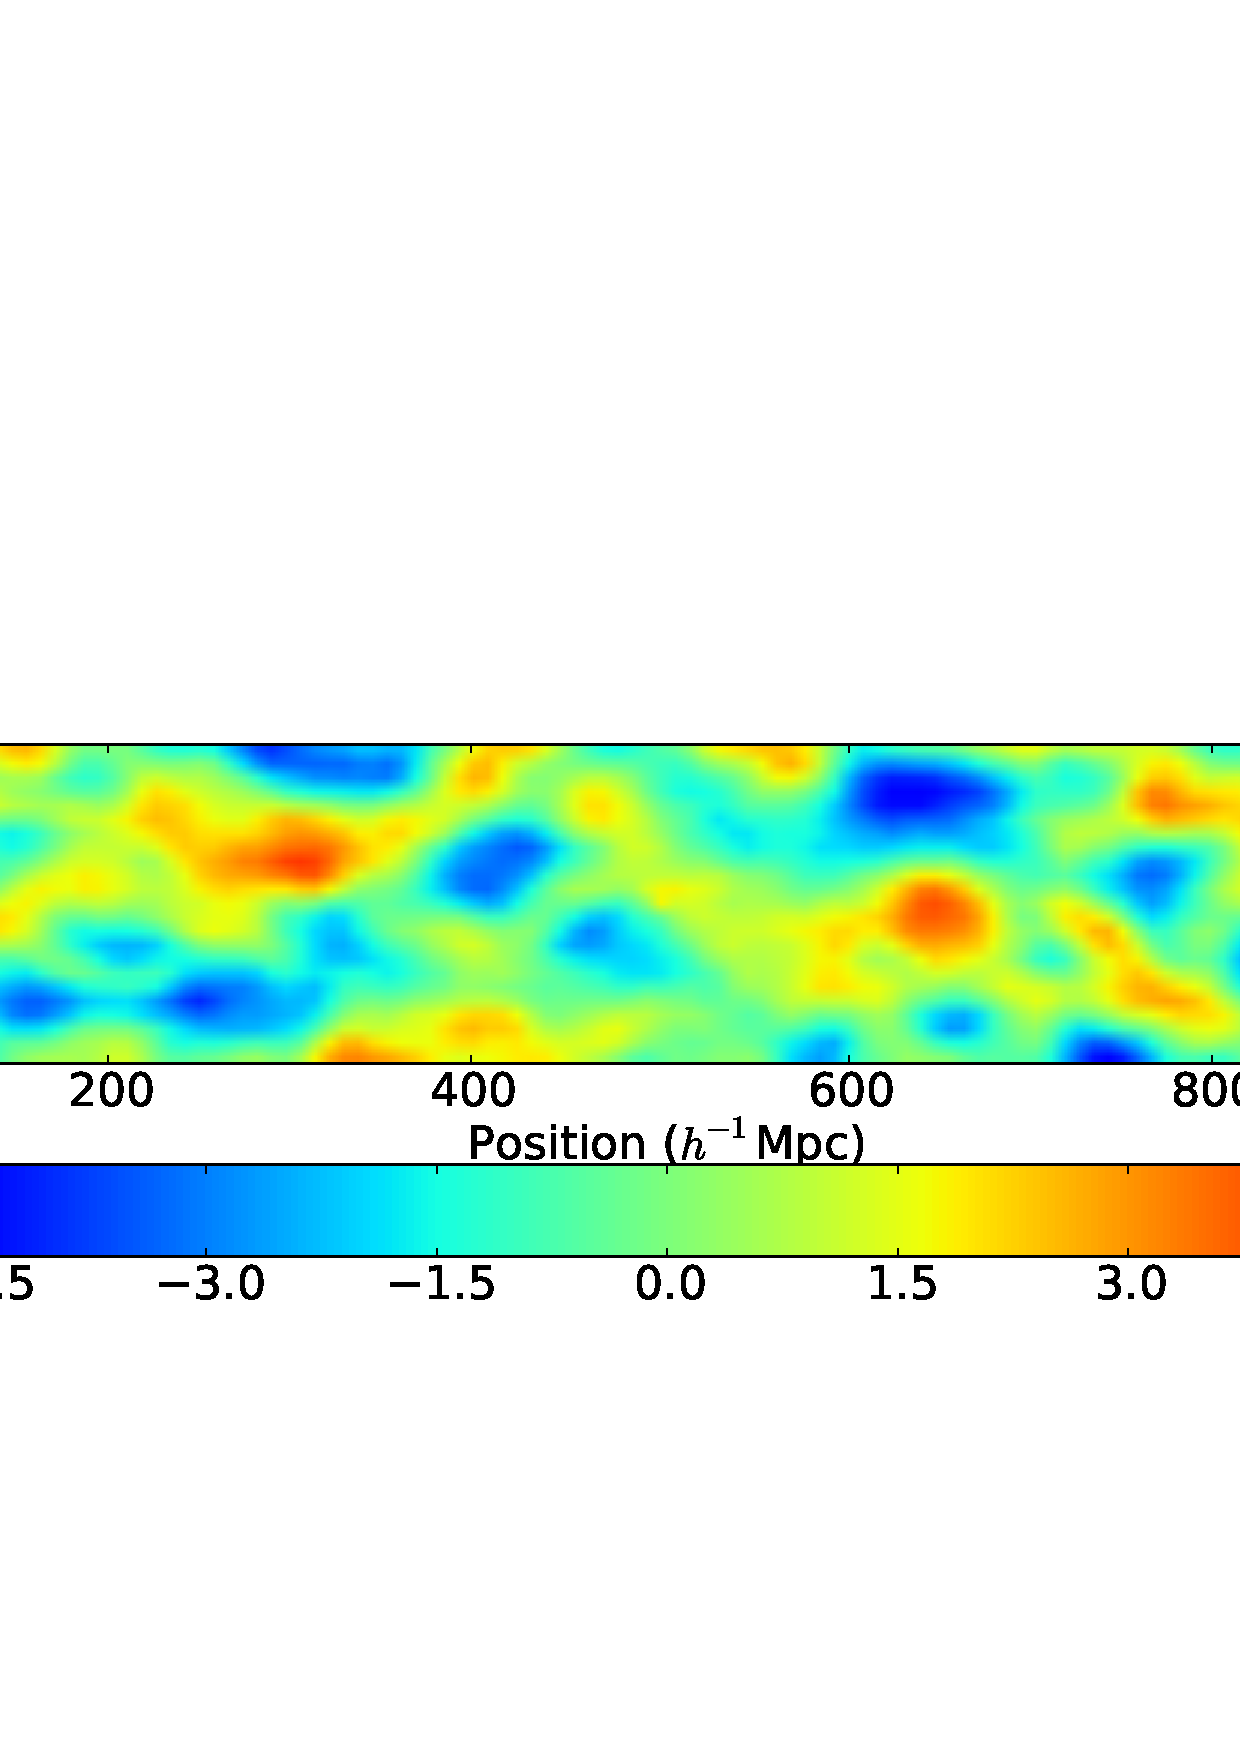
\includegraphics[width=8cm]{f3b.png}
\end{figure}
\end{frame}

\begin{frame}
\frametitle{Toy Model for Detecting Ionized Regions}
\framesubtitle{Isolated, Spherical Bubbles}
\begin{figure}[h]
  \centering
  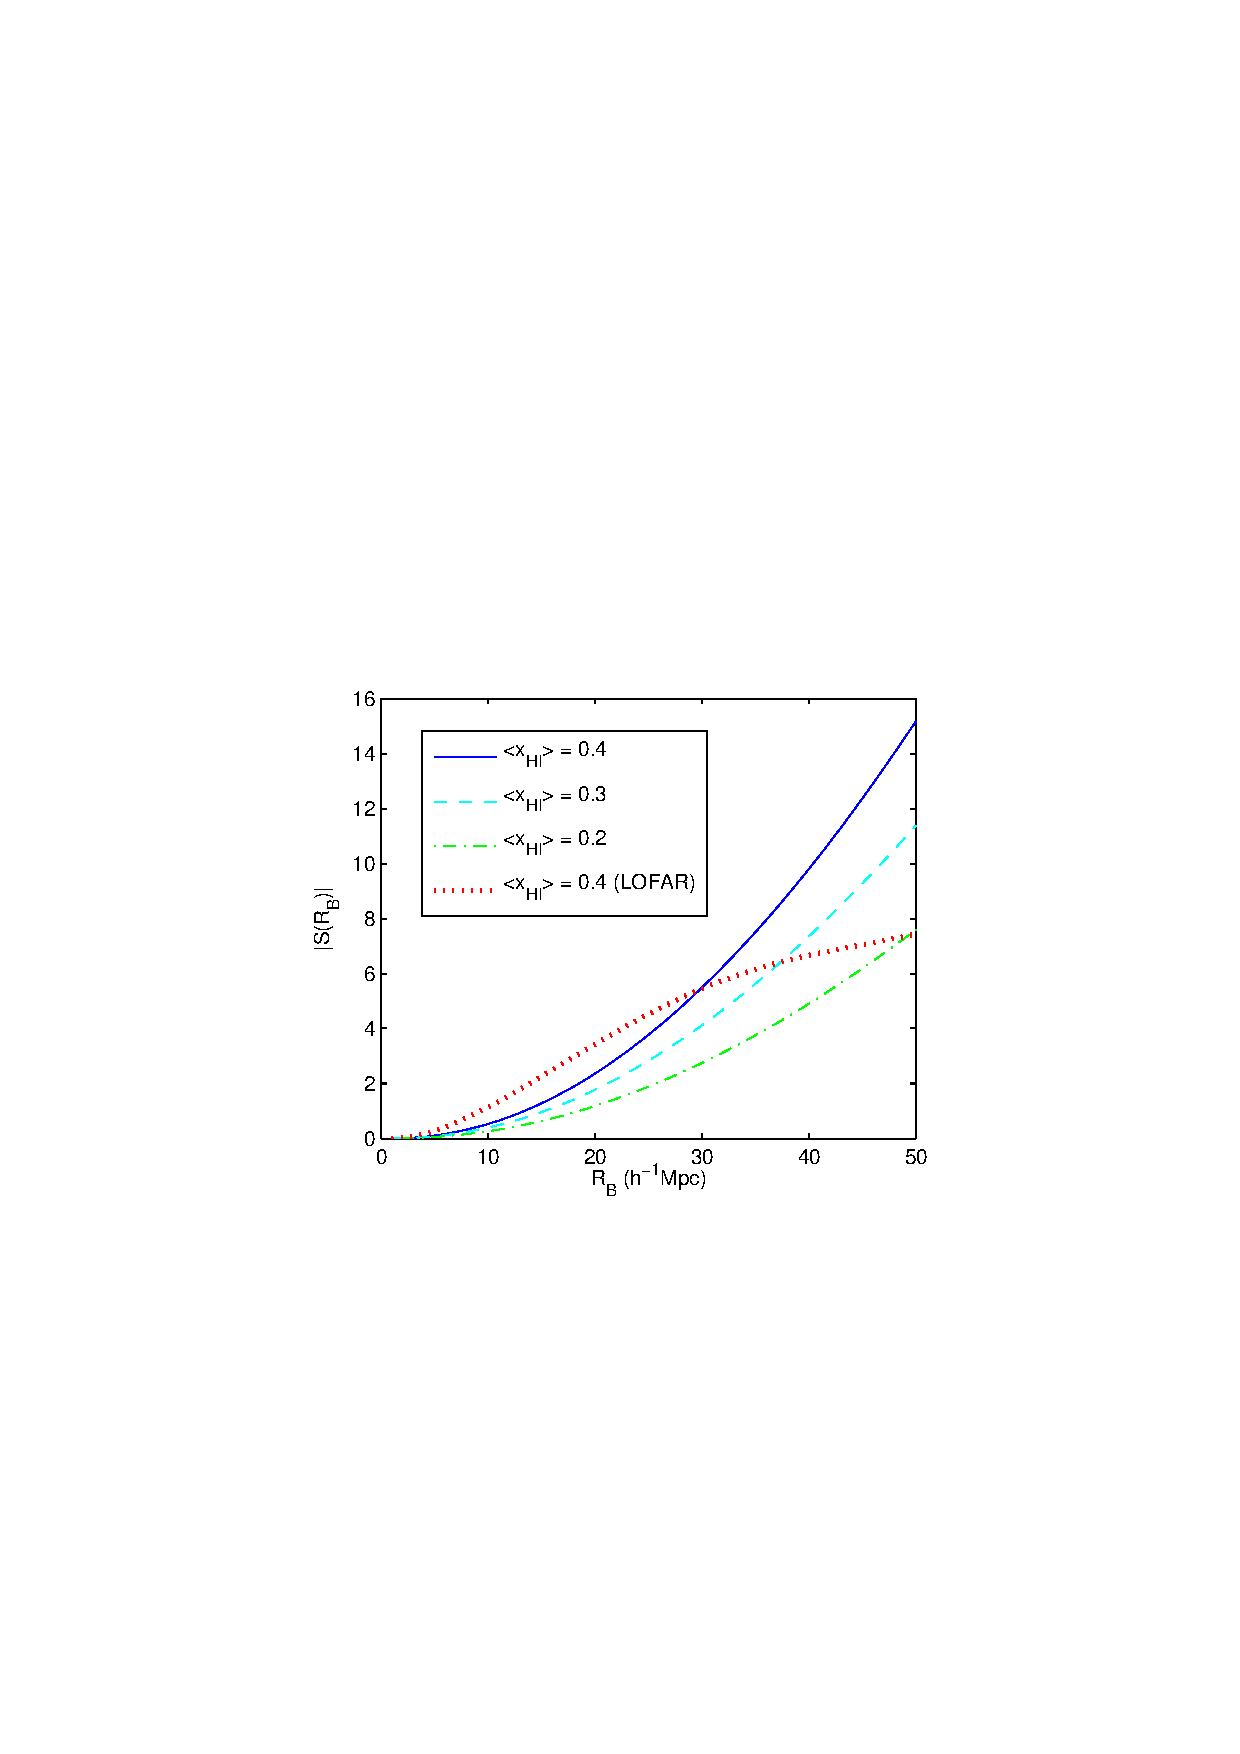
\includegraphics[width=8cm]{f4.png}
\end{figure}
\end{frame}

\begin{frame}
\frametitle{Effects of Foregrounds}
\framesubtitle{Matched Filter}
\begin{figure}[h]
  \centering
  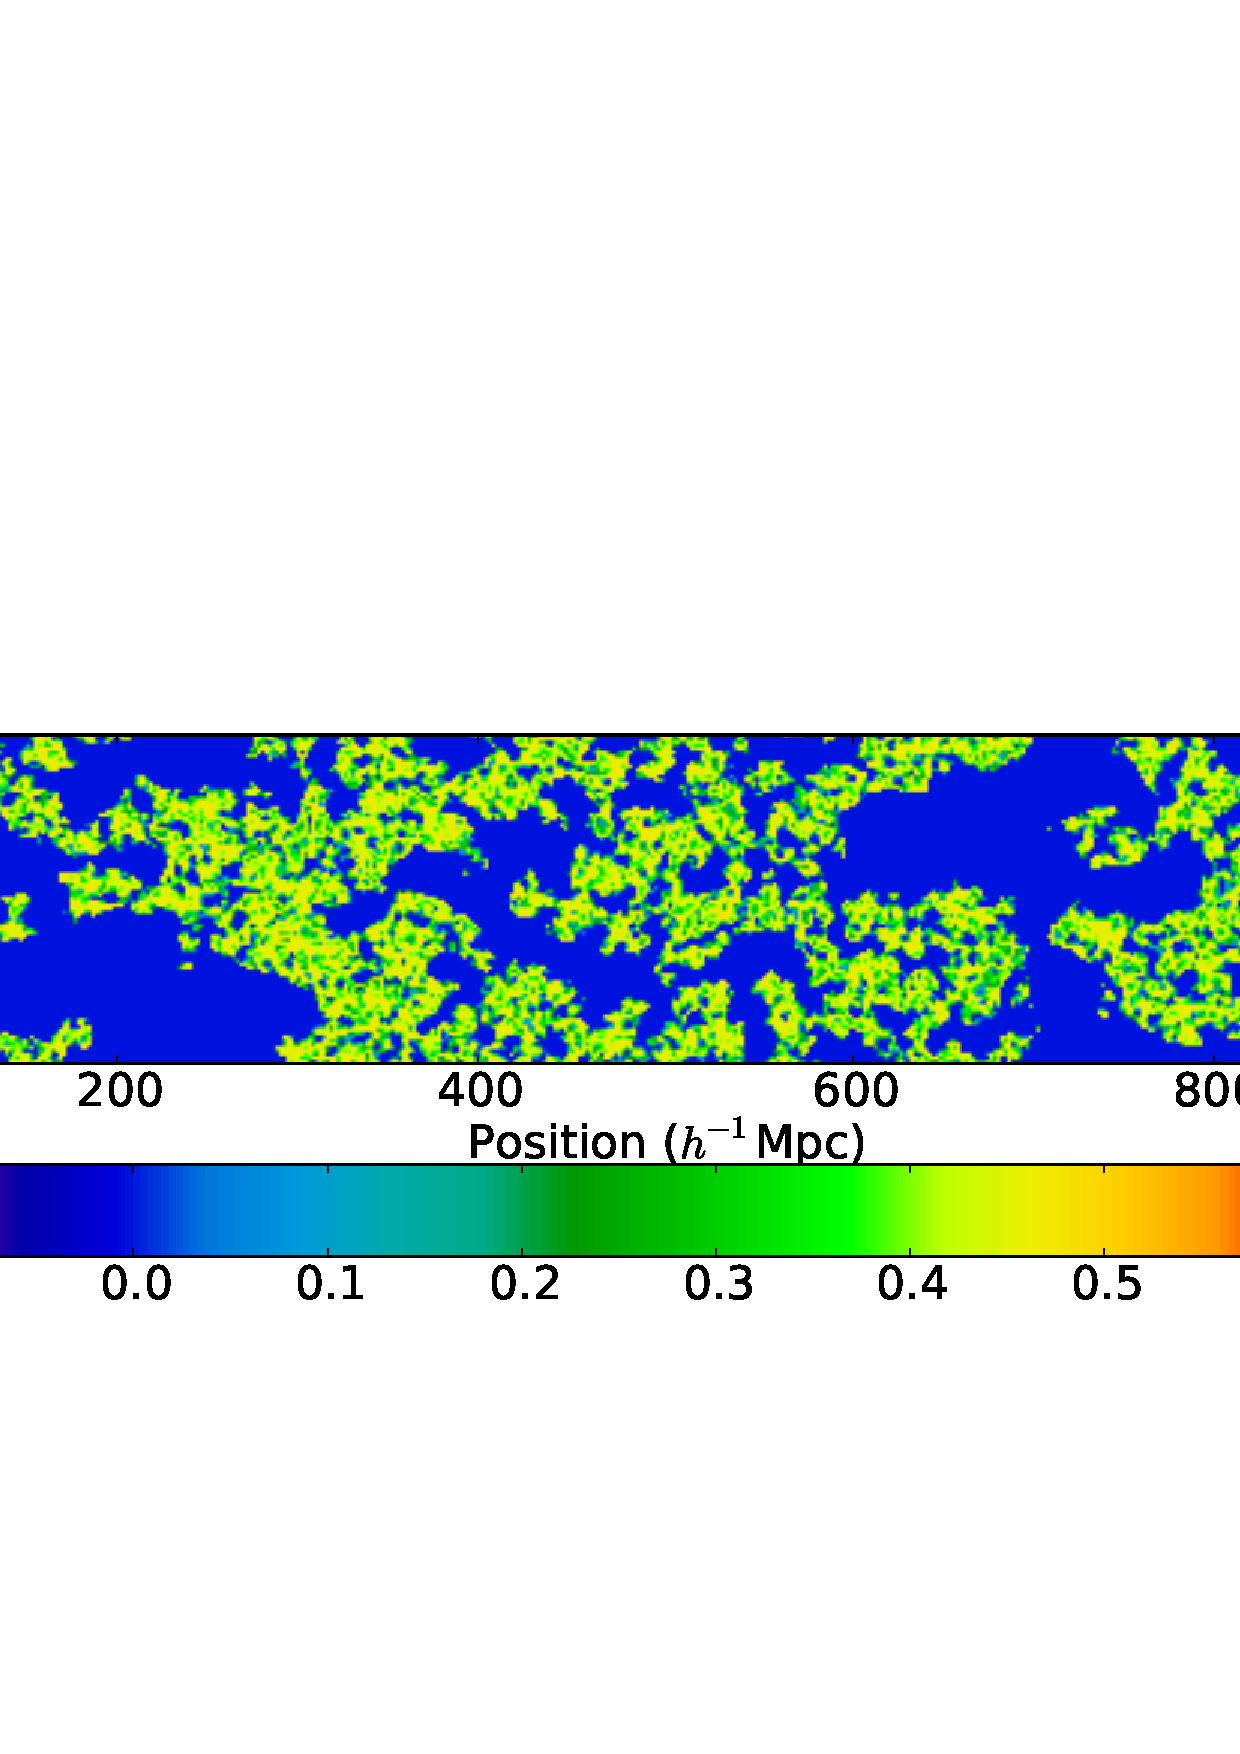
\includegraphics[width=8cm]{f6a.png}\\
  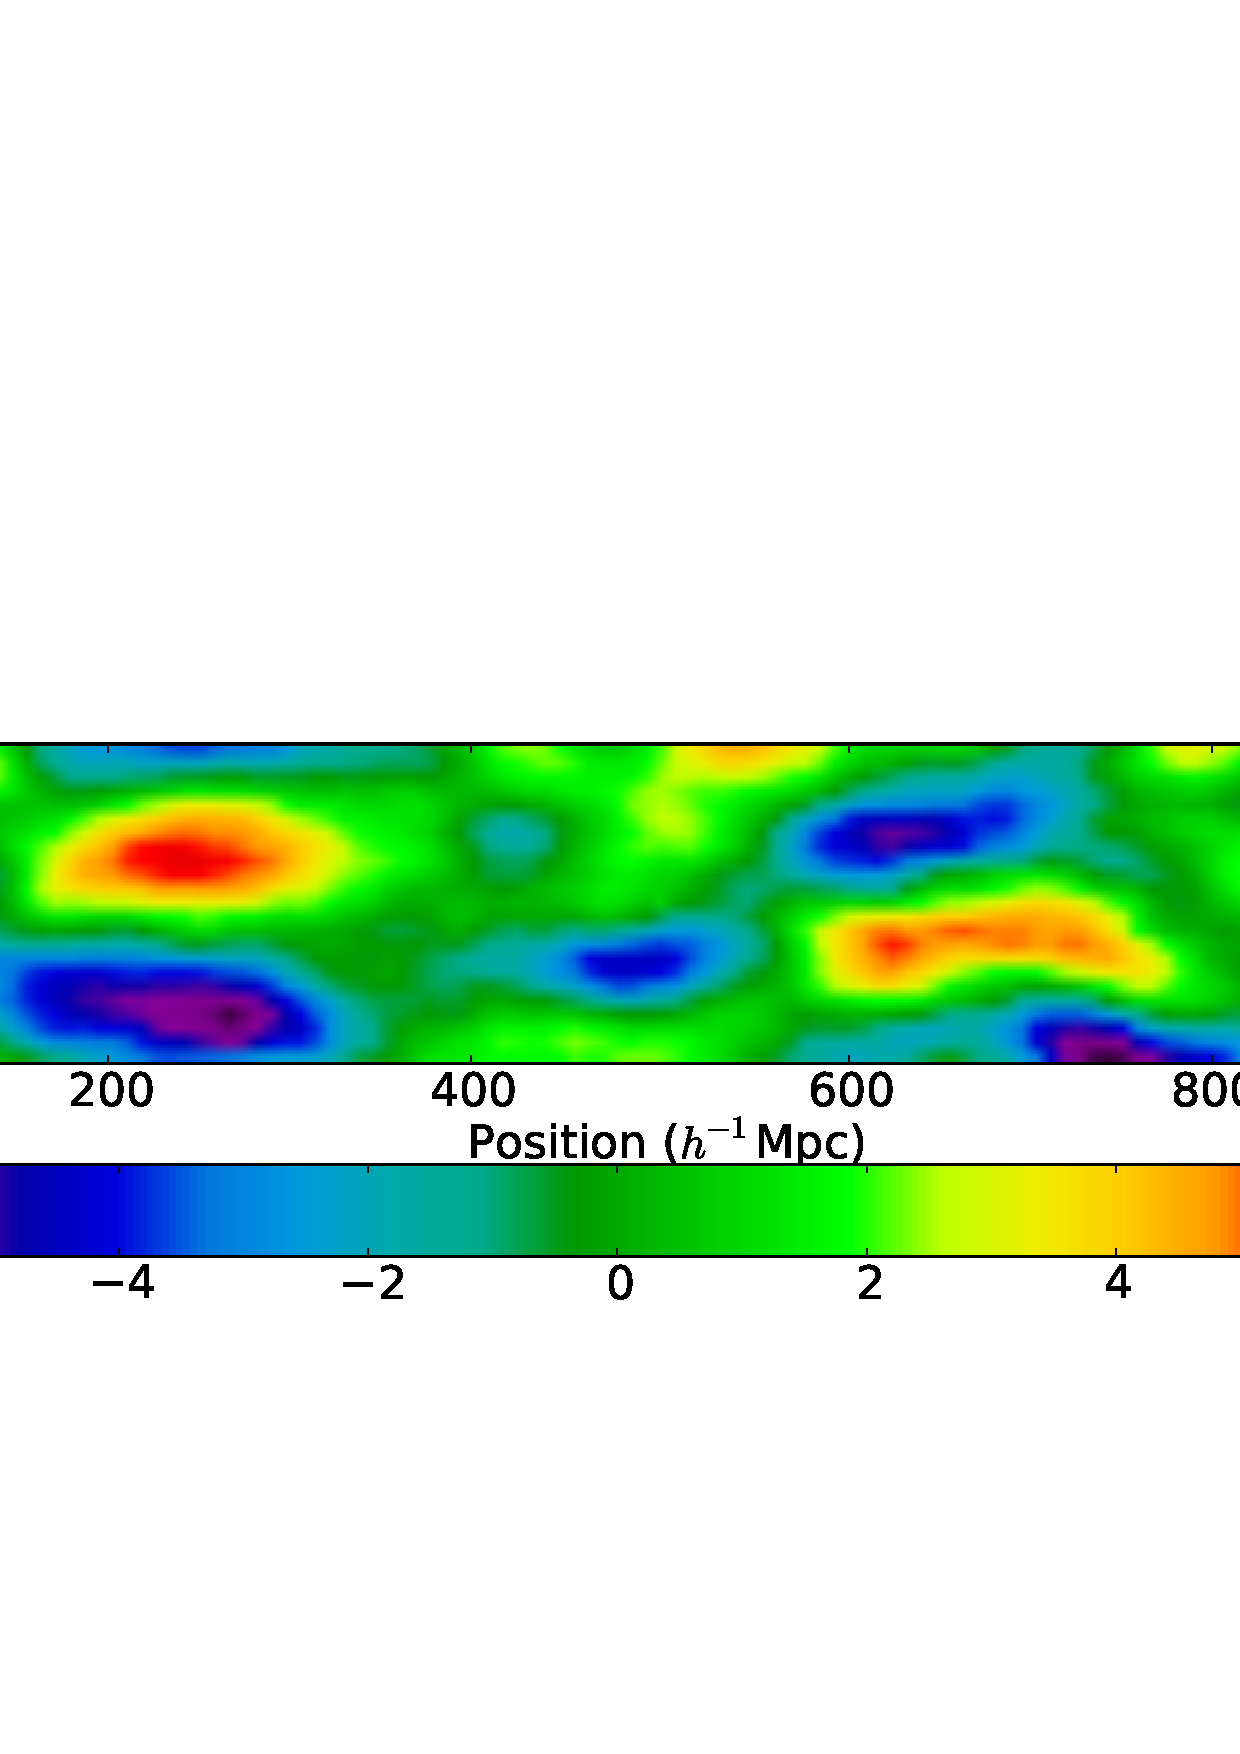
\includegraphics[width=8cm]{f6b.png}
\end{figure}
\end{frame}

\begin{frame}
\frametitle{Detected Bubble Size Distributions}
\framesubtitle{•}
\begin{figure}[h]
  \centering
  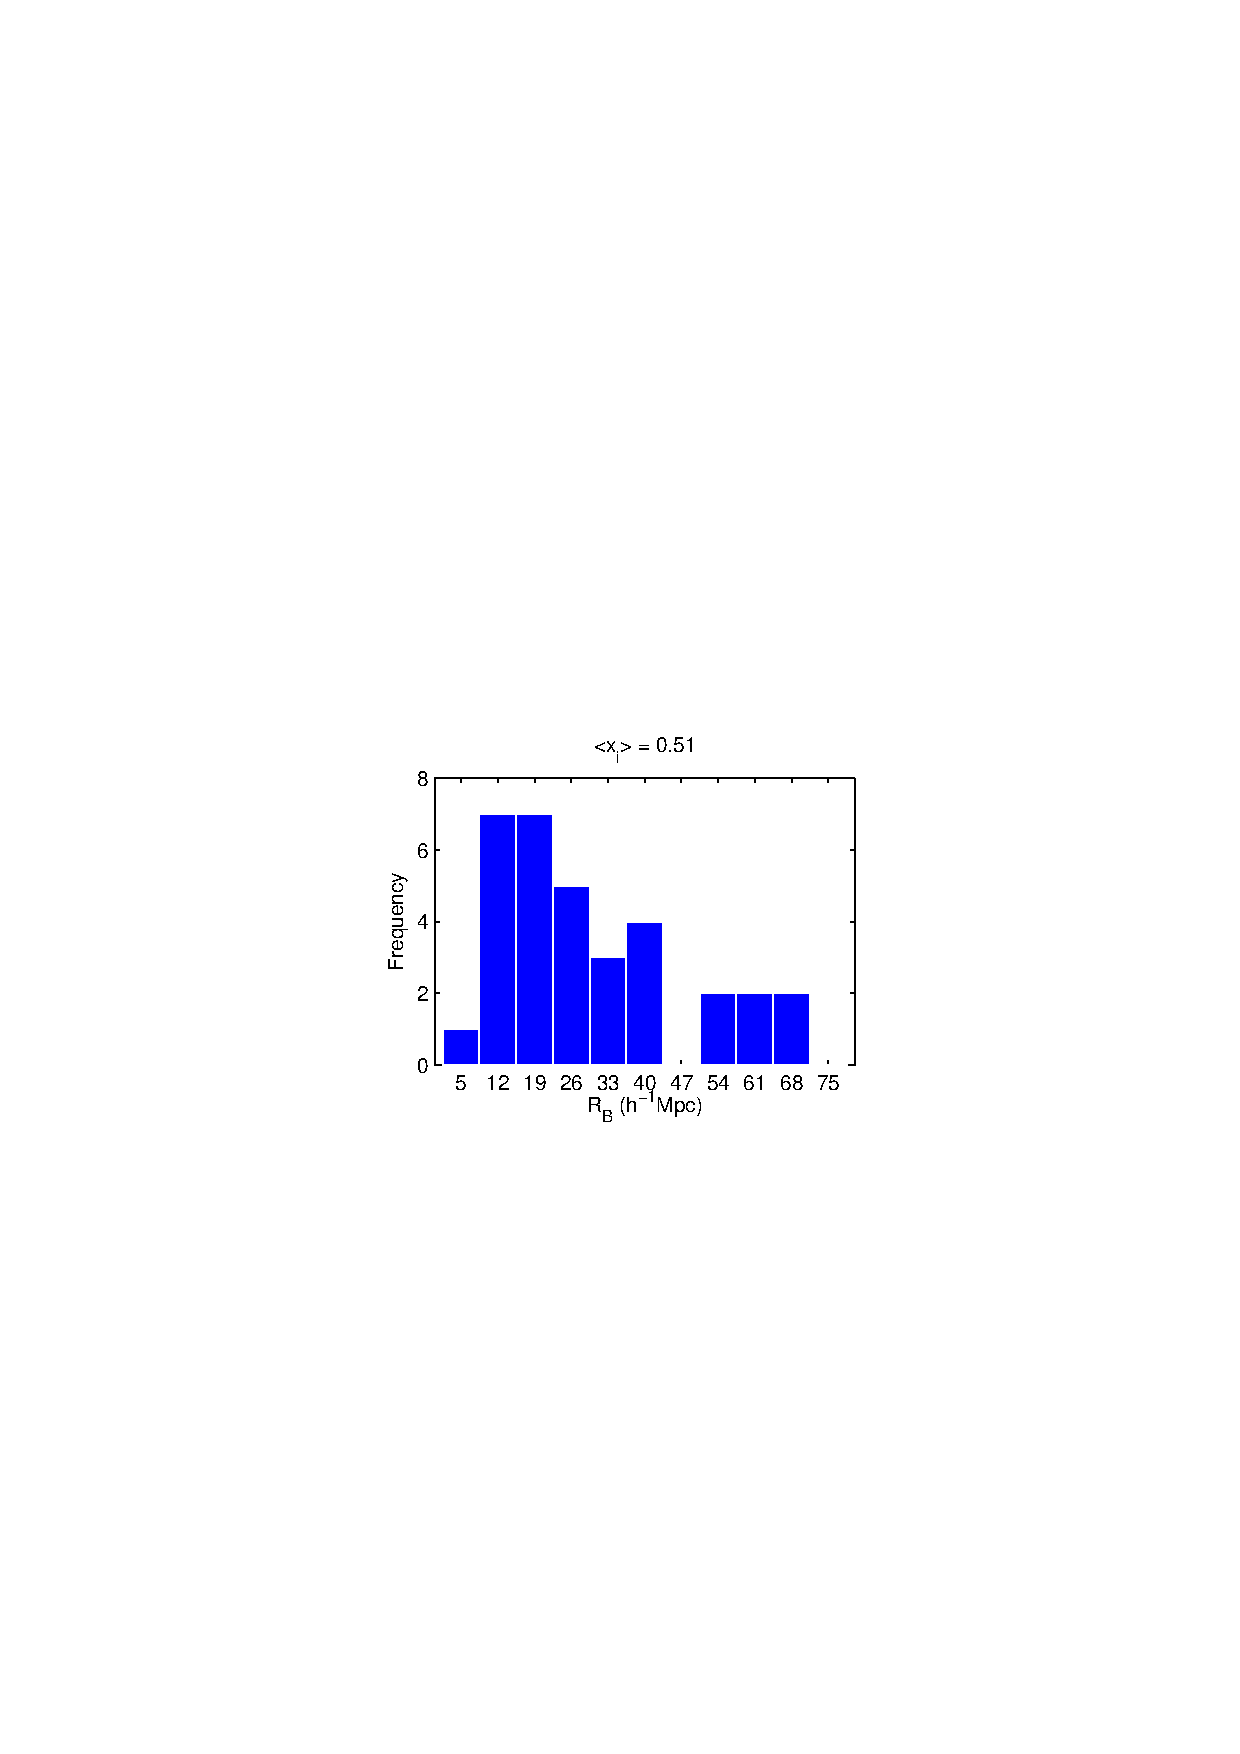
\includegraphics[width=4cm]{f10a.png}
  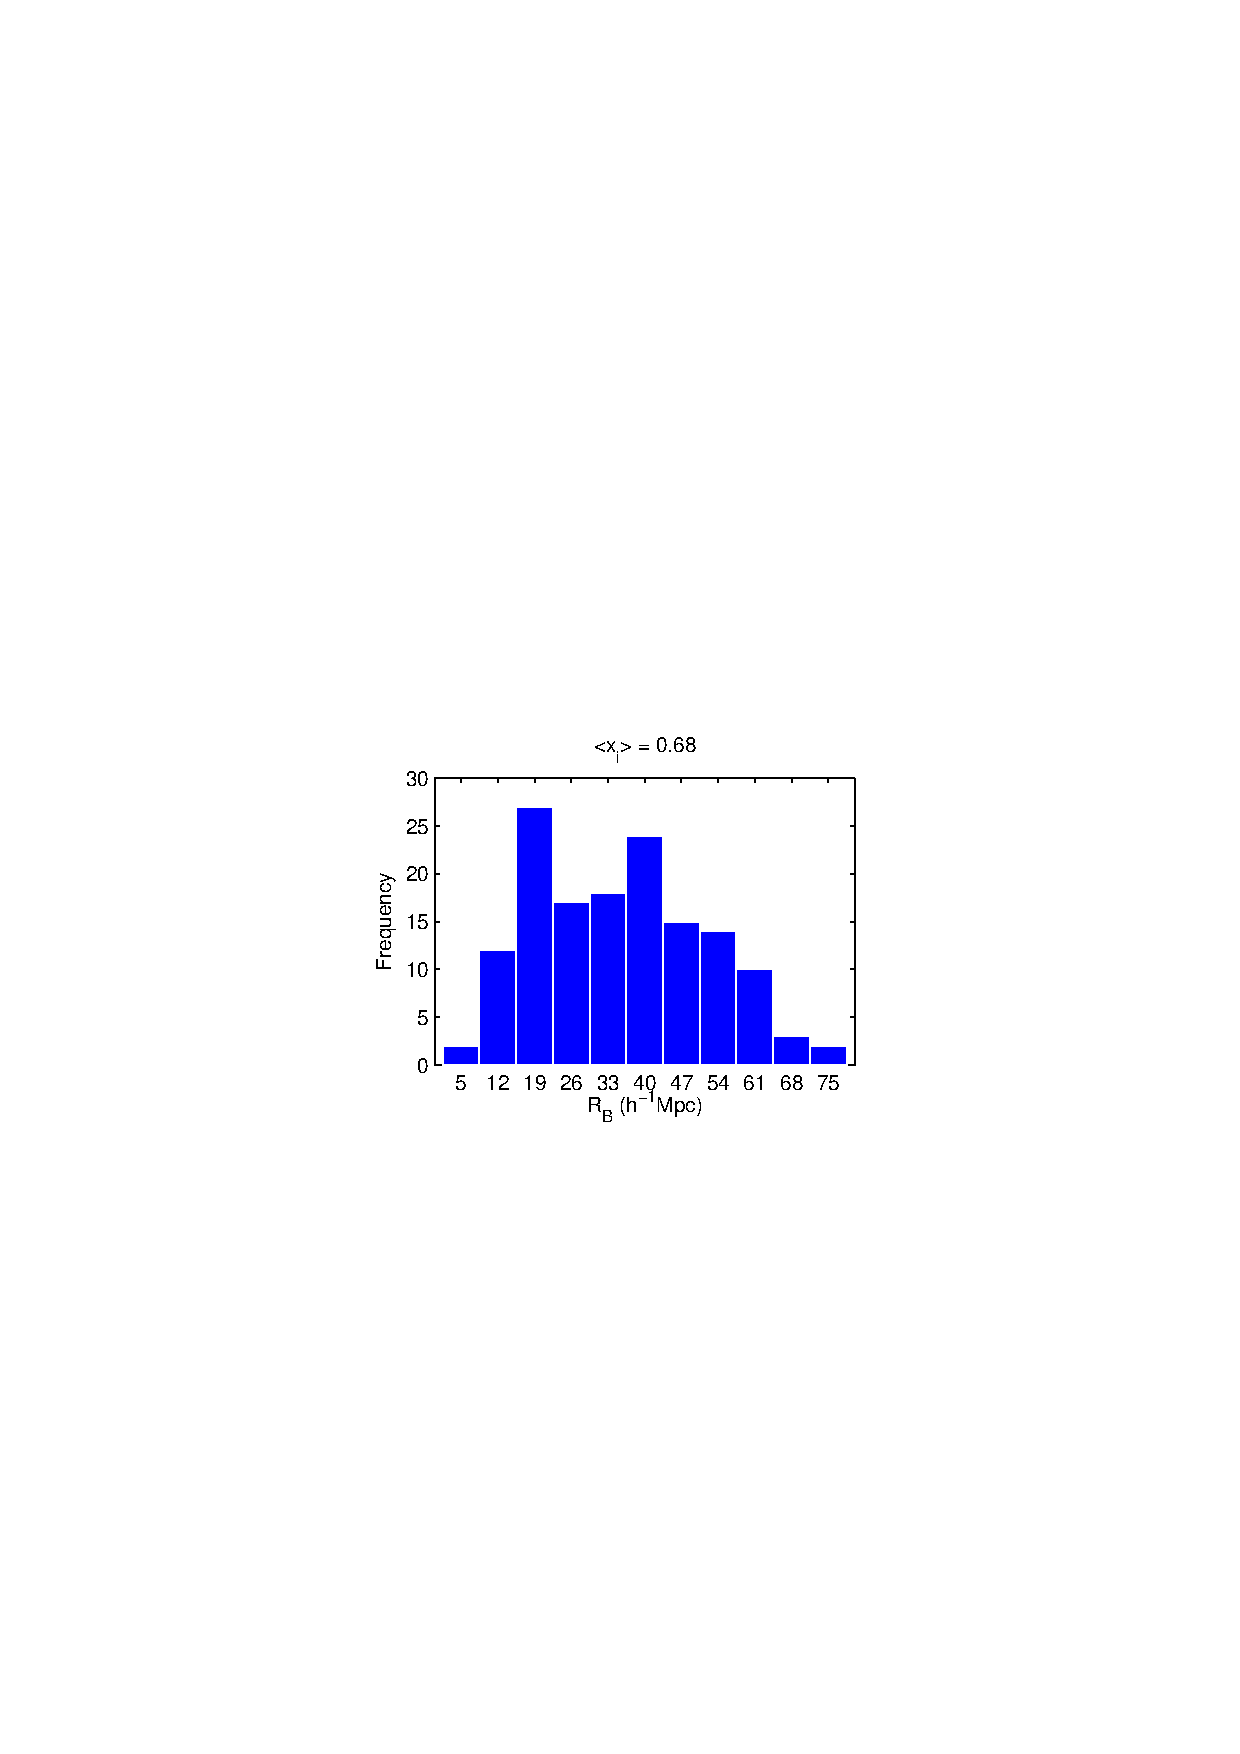
\includegraphics[width=4cm]{f10b.png}\\
  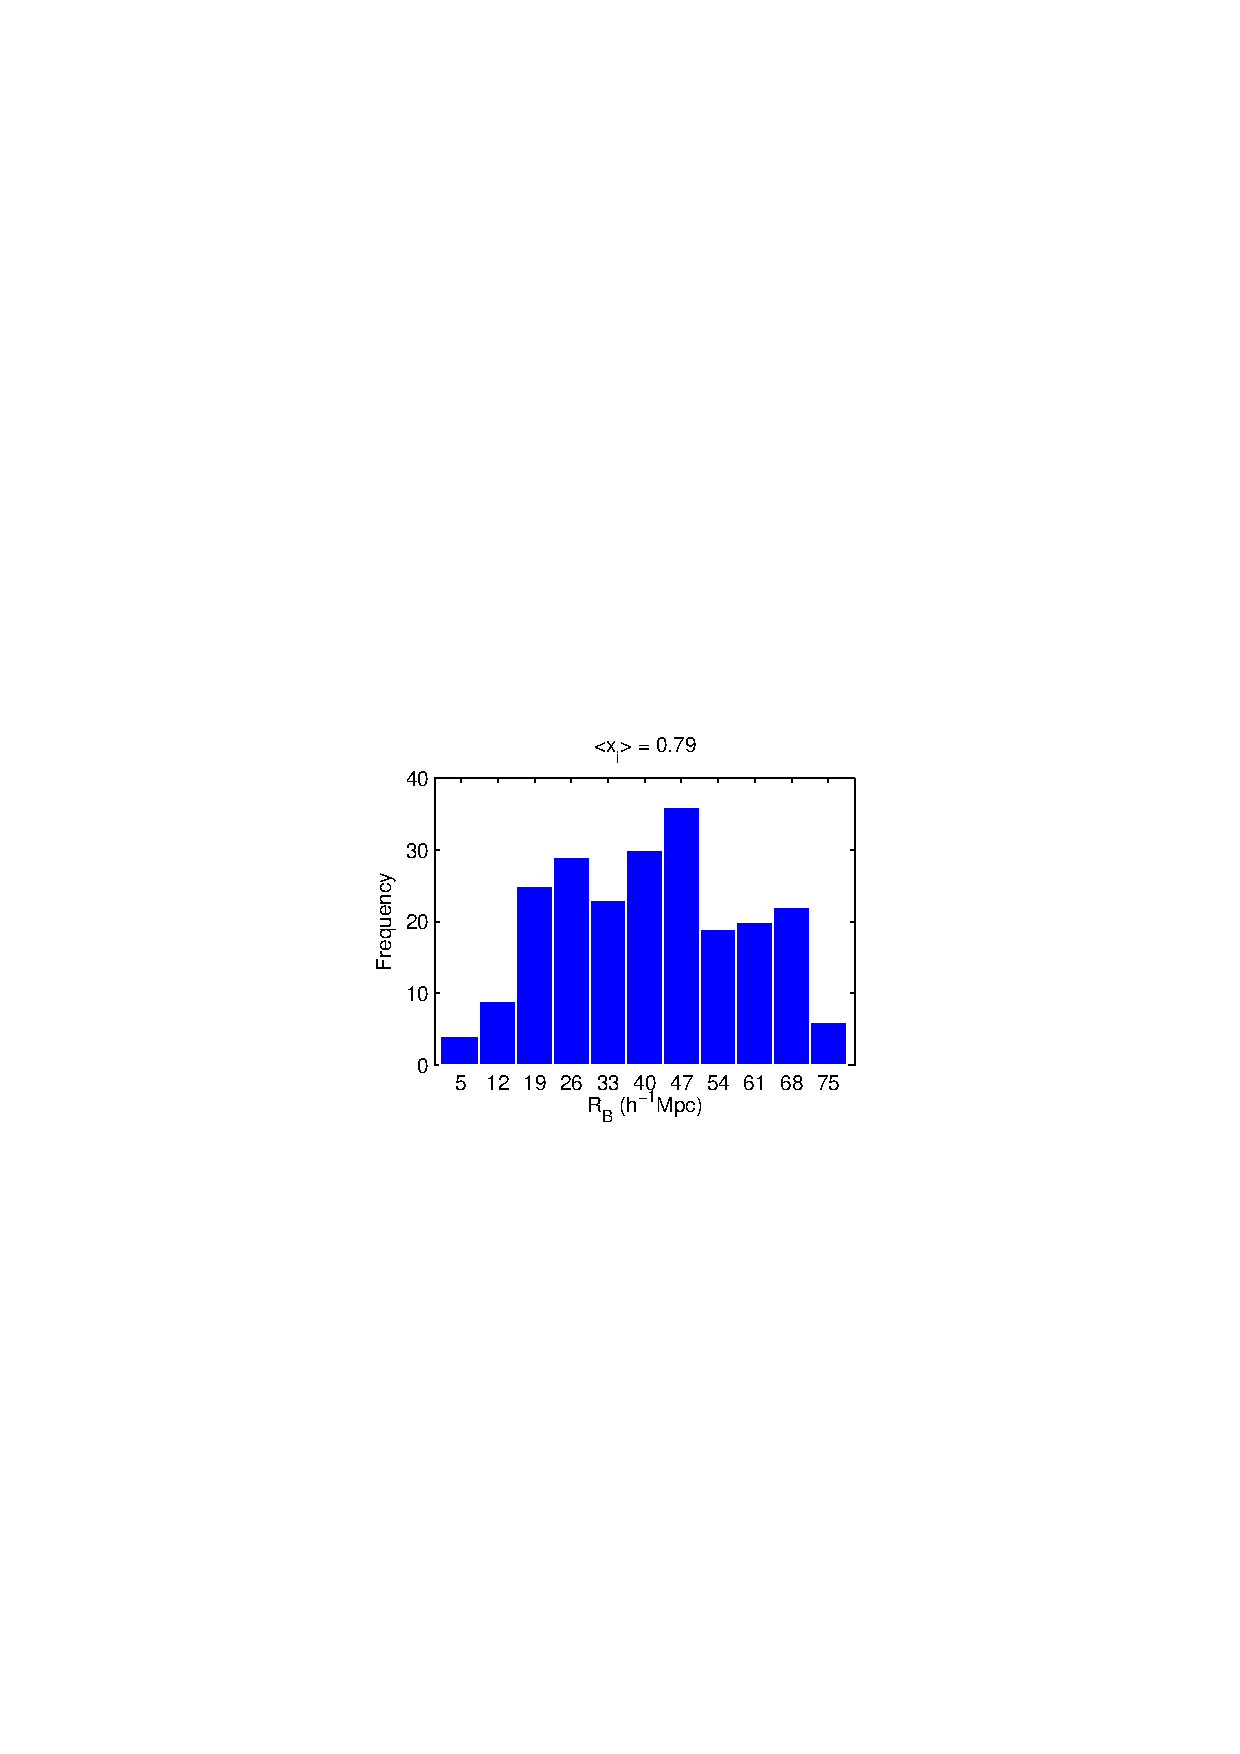
\includegraphics[width=4cm]{f10c.png}
  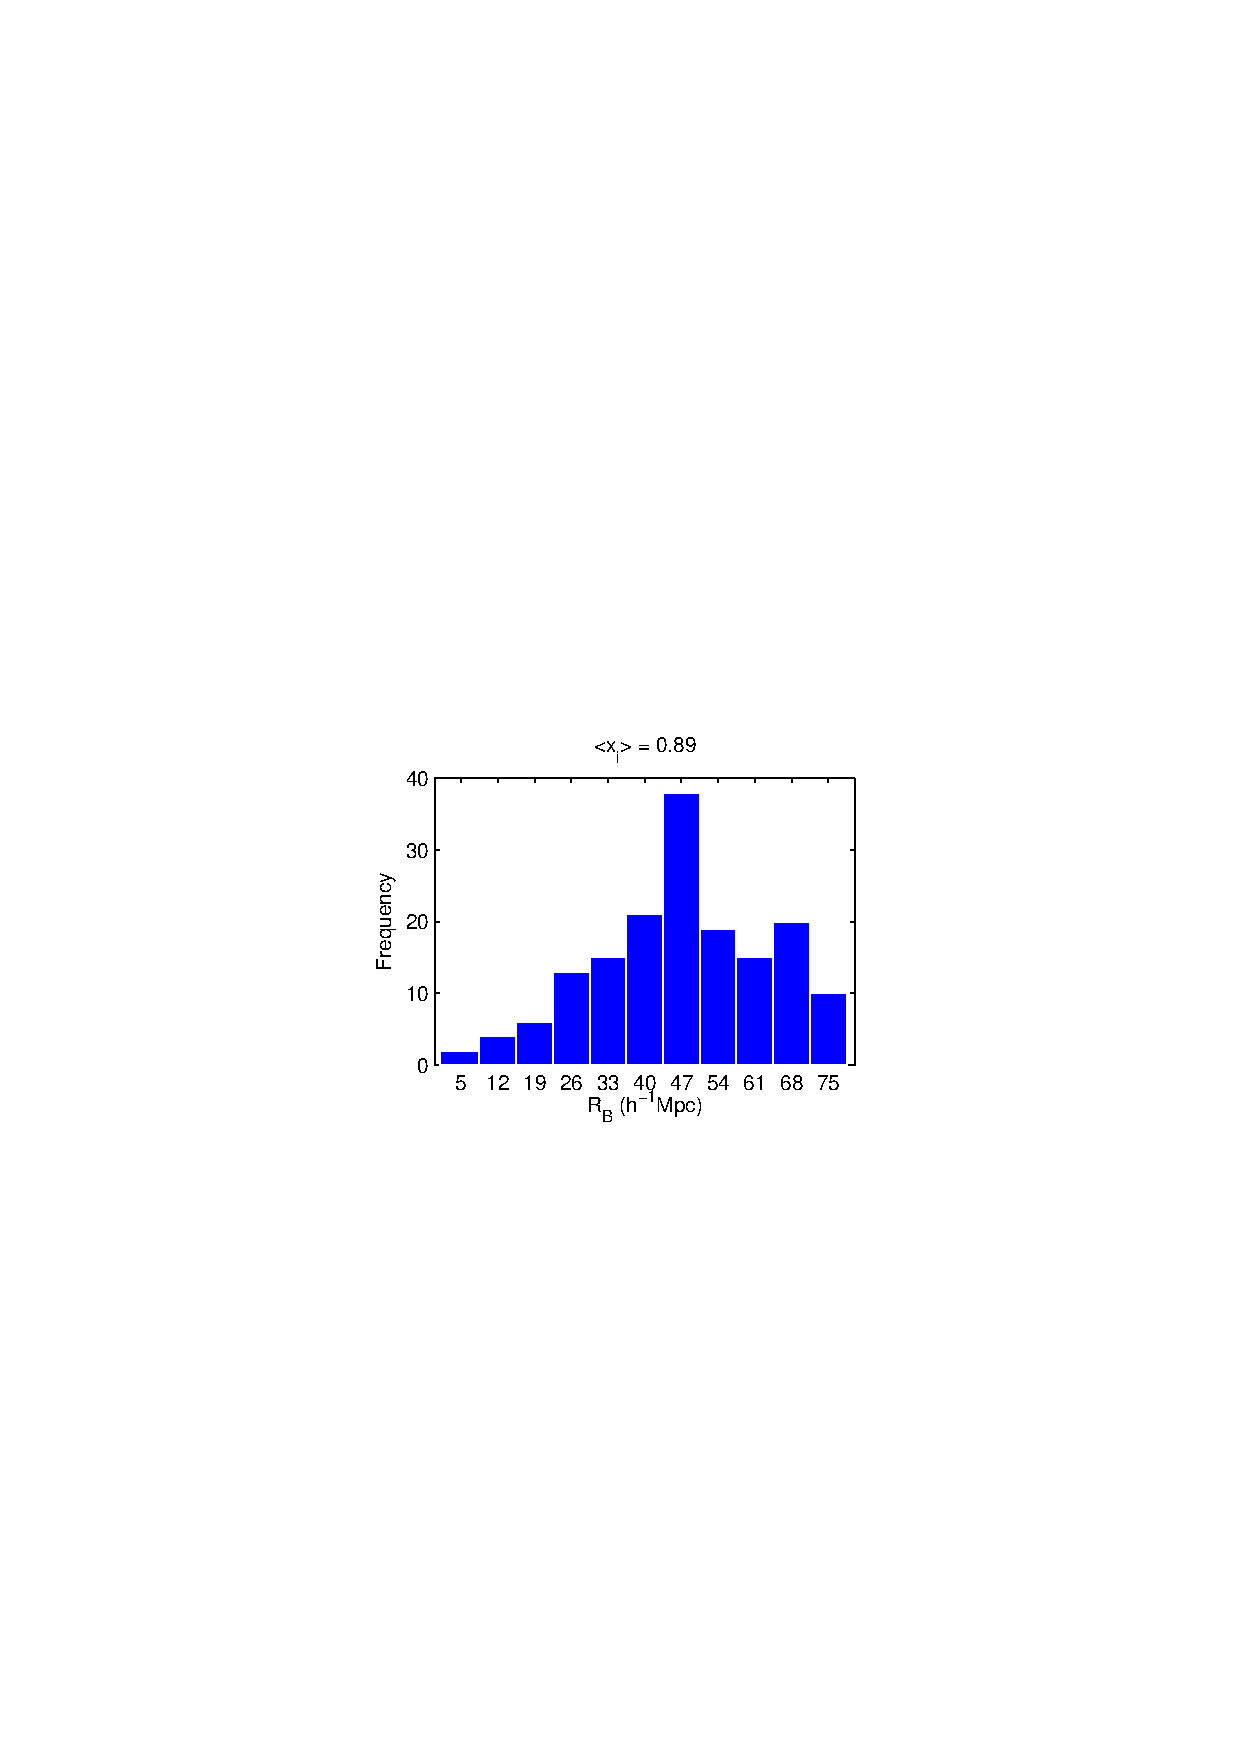
\includegraphics[width=4cm]{f10d.png}
\end{figure}
\end{frame}

\begin{frame}
\frametitle{128-Tile MWA}
\framesubtitle{•}
\begin{figure}[h]
  \centering
  \includegraphics[width=8cm]{f11.png}
\end{figure}
\end{frame}

\begin{frame}
\frametitle{LOFAR}
\framesubtitle{•}
\begin{figure}[h]
  \centering
  \includegraphics[width=8cm]{f12.png}
\end{figure}
\end{frame}

\begin{frame}[noframenumbering]
\frametitle{•}
\framesubtitle{•}
\begin{enumerate}[-]
\item \cite{Fan:2006dp}, \cite{Lidz:2001yc}, Cen \& McDonald (2002), \cite{Furlanetto:2004jz}.
 Fan et al. (2006a)
\end{enumerate}
\end{frame}

\bibliography{matt}
\end{document}






